\mychapter{Expressive Proof Predicates for Multi-Show Attribute-Based (Anonymous) Credentials (ABC's)}


% \begin{table}
% \begin{center}
% \caption{Comparison of our construction over previous work.}
% \label{tab:comparison-chap2}
% \begin{tabular}{l|cccccc}
% Features    									& Multi Issuer & Sybil Resistance  & Revocation & Efficient Cred. Chaining$\footnotemark[1]$ & M-ABC$\footnotemark[2]$   & Anonymity$\footnotemark[3]$   \\
% \hline

% CanDID \cite{maram2021candid}     				& \ding{51}     & \ding{51} 	& \ding{51}  &  \ding{55}     & \ding{55}                     & \ding{55}		\\
% SyRA \cite{crites_syra_2024}     				& \ding{55}     & \ding{51}    	& \ding{55}  &  \ding{55}     & \ding{55}                     & \ding{51}		\\
% S3ID \cite{rabaninejad_attribute-based_2024}  & \ding{51}     & \ding{51}    	& \ding{55}  &  \ding{51}     & \ding{55}\footnotemark[4]     & \ding{51}		\\
% Our Work  										& \ding{51}     & \ding{51}    	& \ding{51}  &  \ding{51}     & \ding{51}                     & \ding{51}		\\
% \end{tabular}
% \end{center}

% \vspace{1em}
% \footnotesize
% $\footnotemark[1]$ Credential Chaining is a user presenting multiple credentials to be verified together for a complex identity statement.

% \footnotesize
% $\footnotemark[2]$ M-ABC is a Multi-Show Attribute Based Credential, allowing a user to satisfy rich, attribute-based identity statements 

% \footnotesize
% $\footnotemark[3]$ Anonymity is defined in the Anonymous Credential model, no verifier and issuer (collaborating together) may learn more about the user or their credentials other than what the user discloses and what their credentials verify. Multiple credential verifications are unlinkable.

% \footnotesize
% $\footnotemark[4]$ While possible in S3ID, they mention 

% \footnotesize
% $\footnotemark[5]$ Multi-issuer means supporting credentials from different authorities that can be cryptographically linked while preserving privacy
% \end{table}

% How can we construct anonymous credential systems that efficiently support expressive proofs—like range proofs, attribute equality, or set membership—while remaining secure against malicious issuers? Existing schemes either verify simple proofs (e.g., possession) efficiently (sps-eq, ACT) or handle complex predicates at high computational cost (zk-creds), often assuming honest issuers (ACT, Coconut). This chapter lays the foundation for a system that overcomes these limitations.

% \noindent \textbf{Technical Challenges}
% \begin{enumerate}
%     \item Formalizing security in the Algebraic Group Model
%     \item Designing an Anonymous Credential scheme for efficient zero-knowledge proof of complex predicates without using zkSNARK
%     \item Ensuring user-anonymity in the presence of malicious issuers without affecting performance
% \end{enumerate}

% \begin{itemize}
%     \item Extended rerandomizable signature scheme with formal position-binding security in the Algebraic Group Model
    % \item Formalized security model for anonymity against colluding credential issuers
%     \item Benchmarked predicate proofs against SOTA showing on average [X\%] improvement
%     \item Provided the first comprehensive benchmarks across BBS+ and PS signature variants
% \end{itemize}

Anonymous credentials represent a fundamental building block for privacy-preserving digital identity, enabling users to prove statements about their attributes without revealing their full identity. Since their introduction by Chaum \cite{chaum_untraceable_1981}, they have evolved from theoretical constructs to practical systems deployed in real-world applications such as U-Prove, Idemix, and PrivacyPass \cite{paquin2011u, camenisch_design_2002, davidson2018privacy}.

The development of anonymous credentials has followed several key advancements:
\begin{itemize}
    \item \textbf{Blind Signatures:} Early constructions using blind signatures provided basic privacy but were limited to single-use scenarios to prevent credential reuse.
    
    \item \textbf{Multi-Show Capabilities:} The introduction of pairing-based signatures \cite{cimato_signature_2003, hutchison_constant-size_2006} enabled efficient multi-show credentials through signature randomization, allowing users to present the same credential multiple times without being linked.
    
    \item \textbf{Attribute-Based Credentials and Expressive Proofs:} Modern systems extend beyond simple possession proofs to enable selective disclosure and complex predicate verification over attributes.
\end{itemize}

Despite these advances, current attribute-based anonymous credential (ABC) systems face a critical trade-off between expressiveness and efficiency. Systems like SPS-EQ \cite{fuchsbauer_structure-preserving_2019, hanaoka_improved_2022} and ACT \cite{guo_anonymous_2023} achieve high efficiency but support only limited predicates, while approaches based on zkSNARKs enable rich expressiveness \cite{rosenberg_zk-creds_2022} but at computational cost. Furthermore, many anonymous credential systems assume honest issuers, leaving users vulnerable to privacy breaches from malicious credential providers.

This chapter addresses these limitations through four key contributions:
\begin{enumerate}
    \item \textbf{Extended Rerandomizable Signature Scheme:} We build upon the foundations in \cite{tomescu2022utt} to develop a rerandomizable signature scheme over commitments, proven secure in the Algebraic Group Model (AGM) and satisfies the Anonymous Credential System model from \cite{fuchsbauer_structure-preserving_2019}.
    
    \item \textbf{Optimized Verification Construction:} Our optimized signature variant reduces show/verify costs by X\% compared to previous approaches

    \item \textbf{Optimized Expressive Proofs:} Compared to snarkbased proofs, we show ours reduces show/verify time by X\%
    
    \item \textbf{Formalized Security Against Malicious Issuers:} We provide a comprehensive security model that guarantees user privacy even against colluding credential issuers, addressing a critical limitation in existing systems.
    
    \item \textbf{Empirical Performance Validation:} We benchmark against state-of-the-art alternatives, and we demonstrate that schnorr proofs, as used in our construction, are, in fact, sub-linear in practice and fully expressive for predicate proofs.
\end{enumerate}

These foundations support the multi-issuer, multi-credential system presented in subsequent chapters while maintaining security against malicious issuers and offering practical performance for real-world applications.


\subsubsection*{Chapter Roadmap}
The remainder of this chapter is organized as follows: Section 2.1 presents preliminaries and notation. Section 2.2 introduces our position-binding commitment scheme. Section 2.3 details our rerandomizable signature construction. Section 2.4 presents our attribute-based credential system construction. Section 2.5 provides comprehensive performance evaluations, and Section 2.6 summarizes our findings.


















\newpage
\section{Preliminaries}

\begin{definition}[Signature Scheme]
A signature scheme $\mathsf{Sig}$ is a tuple of probabilistic polynomial-time algorithms $(\mathsf{KeyGen}, \mathsf{Sign}, \mathsf{Verify})$ where:

\begin{itemize}
    \item $\mathsf{KeyGen}(1^\lambda) \rightarrow (\mathsf{sk}, \mathsf{pk})$: is a probabilistic algorithm that takes as input a security parameter $\lambda$ and outputs a secret signing key $\mathsf{sk}$ and a public verification key $\mathsf{pk}$. The message space $\mathcal{M}$ is implicitly defined by $\mathsf{pk}$.
    
    \item $\mathsf{Sign}(\mathsf{sk}, m; r) \rightarrow \sigma$: is a probabilistic algorithm that takes as input the secret key $\mathsf{sk}$, a message $m \in \mathcal{M}$, and random coins $r$ sampled from the randomness space $\mathcal{R}$. It outputs a signature $\sigma$.
    
    \item $\mathsf{Verify}(\mathsf{pk}, m, \sigma) \rightarrow b$: is a deterministic algorithm that takes as input the public key $\mathsf{pk}$, a message $m \in \mathcal{M}$, and a signature $\sigma$. It outputs a bit $b \in \{0,1\}$, where 1 indicates acceptance and 0 indicates rejection.
\end{itemize}

\end{definition}

\begin{definition}[Correctness]
A signature scheme $(\mathsf{KeyGen}, \mathsf{Sign}, \mathsf{Verify})$ is correct if for all $k \in \mathbb{N}$, all key pairs $(\mathsf{sk}, \mathsf{pk}) \in [\mathsf{KeyGen}(1^k)]$ and all $m \in \mathcal{M}$ we have:

$$\Pr[\mathsf{Verify}(m, \mathsf{Sign}(m, \mathsf{sk}), \mathsf{pk}) = 1] = 1.$$
\end{definition}

\begin{definition}[EUF-CMA Security]
A signature scheme $(\mathsf{KeyGen}, \mathsf{Sign}, \mathsf{Verify})$ is existentially unforgeable under adaptive chosen-message attacks if for all PPT algorithms $\mathcal{A}$, there exists a negligible function $\negl$ such that:
$$\Pr\left[\begin{array}{l}
    (\mathsf{sk}, \mathsf{pk}) \sample \mathsf{KeyGen}(1^\lambda) \\
    (m^*, \sigma^*) \sample \mathcal{A}^{\mathcal{O}_{\mathsf{sk}}}(\mathsf{pk})
\end{array} : \begin{array}{l}
    m^* \notin Q \land \\
    \mathsf{Verify}(m^*, \sigma^*, \mathsf{pk}) = 1
\end{array}\right] \leq \negl$$
where $Q$ is the set of queries made to $\mathcal{O}_{\mathsf{sk}}$ with access to $\mathsf{sk}$ is defined by:
\[
\text{Oracle }\mathcal{O}_{\mathsf{sk}}(m): \text{ Returns } \sigma \gets \mathsf{Sign}(m, \mathsf{sk})
\]
\end{definition}

\begin{definition}[Commitment Scheme]\label{def:commitmentscheme}
A commitment scheme $\mathsf{Com}$ is a tuple of probabilistic polynomial-time algorithms $(\mathsf{Setup}, \mathsf{Commit}, \mathsf{Open})$ where:
\begin{itemize}
    \item $\mathsf{Setup}(1^\lambda) \rightarrow \mathsf{ck}$: is a probabilistic algorithm that takes as input a security parameter $\lambda$ and outputs a commitment key $\mathsf{ck}$. The message space $\mathcal{M}$ is implicitly defined by $\mathsf{ck}$.
    
    \item $\mathsf{Commit}(\mathsf{ck}, m) \rightarrow (\mathsf{cm}, r)$: is a probabilistic algorithm that takes as input the commitment key $\mathsf{ck}$ and a message $m \in \mathcal{M}$. It outputs a commitment $\mathsf{cm}$ and an opening value $r$.
    
    \item $\mathsf{Open}(\mathsf{ck}, \mathsf{cm}, m, r) \rightarrow b$: is a deterministic algorithm that takes as input the commitment key $\mathsf{ck}$, a commitment $\mathsf{cm}$, a message $m$, and an opening value $r$. It outputs a bit $b \in \{0,1\}$, where 1 indicates a valid opening and 0 indicates an invalid opening.
\end{itemize}
\end{definition}

\begin{definition}[Correctness]
A commitment scheme $(\mathsf{Setup}, \mathsf{Commit}, \mathsf{Open})$ is correct if for all $\lambda \in \mathbb{N}$, all commitment keys $\mathsf{ck} \in [\mathsf{Setup}(1^\lambda)]$, and all messages $m \in \mathcal{M}$:
$$\Pr[(\mathsf{cm}, r) \sample \mathsf{Commit}(\mathsf{ck}, m) : \mathsf{Open}(\mathsf{ck}, \mathsf{cm}, m, r) = 1] = 1.$$
\end{definition}

\begin{definition}[Hiding]
A commitment scheme $(\mathsf{Setup}, \mathsf{Commit}, \mathsf{Open})$ is hiding if for all PPT adversaries $\mathcal{A}$, there exists a negligible function $\negl$ such that:
$$\left|\Pr\left[\begin{array}{l}
    \mathsf{ck} \sample \mathsf{Setup}(1^\lambda) \\
    (m_0, m_1) \sample \mathcal{A}(\mathsf{ck}) \\
    b \sample \{0,1\} \\
    (\mathsf{cm}, r) \sample \mathsf{Commit}(\mathsf{ck}, m_b) \\
    b' \sample \mathcal{A}(\mathsf{ck}, \mathsf{cm})
\end{array} : b' = b\right] - \frac{1}{2}\right| \leq \negl(\lambda)$$
\end{definition}

\begin{definition}[Binding]
A commitment scheme $(\mathsf{Setup}, \mathsf{Commit}, \mathsf{Open})$ is binding if for all PPT adversaries $\mathcal{A}$, there exists a negligible function $\negl$ such that:
$$\Pr\left[\begin{array}{l}
    \mathsf{ck} \sample \mathsf{Setup}(1^\lambda) \\
    (\mathsf{cm}, m_0, m_1, r_0, r_1) \sample \mathcal{A}(\mathsf{ck})
\end{array} : \begin{array}{l}
    m_0 \neq m_1 \land \\
    \mathsf{Open}(\mathsf{ck}, \mathsf{cm}, m_0, r_0) = 1 \land \\
    \mathsf{Open}(\mathsf{ck}, \mathsf{cm}, m_1, r_1) = 1
\end{array}\right] \leq \negl(\lambda)$$
\end{definition}

\subsubsection{Zero-Knowledge Proofs}
A zero-knowledge proof (ZKP) enables a prover $\mathcal{P}$ to convince a verifier $\mathcal{V}$ that a statement $x \in L$ holds for some language $L$, without revealing the witness $w$. Formally, an interactive proof system $(\mathcal{P}, \mathcal{V})$ for $L$ satisfies:
\begin{itemize}
    \item \textbf{Completeness}: If $x \in L$, then $\Pr[(\mathcal{P}(w), \mathcal{V})(x) = 1] \geq 1 - \negl(\lambda)$.
    \item \textbf{Soundness}: If $x \notin L$, then for any $\mathcal{P}^*$, $\Pr[(\mathcal{P}^*, \mathcal{V})(x) = 1] \leq \negl(\lambda)$.
    \item \textbf{Zero-Knowledge}: There exists a simulator $\mathcal{S}$ such that for all $x \in L$, the view of any $\mathcal{V}^*$ is computationally indistinguishable from $\mathcal{S}(x)$.
\end{itemize}
ZKPs are essential to our anonymous credential system, allowing users to prove credential validity and attribute relations without compromising privacy.

\subsubsection{Sigma-Protocols}
A Sigma-protocol is a three-move, public-coin ZKP: (1) $\mathcal{P}$ sends a commitment $a$, (2) $\mathcal{V}$ sends a random challenge $e$, and (3) $\mathcal{P}$ responds with $z$. It satisfies:
\begin{itemize}
    \item \textbf{Completeness}: Honest execution accepts with probability 1.
    \item \textbf{Special Soundness}: From two accepting transcripts $(a, e, z)$ and $(a, e', z')$ with $e \neq e'$, a witness $w$ can be extracted.
    \item \textbf{Special Honest-Verifier Zero-Knowledge (SHVZK)}: A simulator can generate transcripts $(a, e, z)$ matching the real distribution for any $e$.
\end{itemize}
We leverage Sigma-protocols to prove knowledge of committed attributes (e.g., $\pircom$ for relation $\rcom$) efficiently. app:zkp for details. %See Appendix~\ref{app:zkp}

\subsection{Assumptions}


\begin{definition}[Symmetric Discrete Logarithm Assumption (SDLP)]\label{sdlp}
For any PPT adversary $\mathcal{A}$, we say the SDLP assumption holds if there exists a negligible function $\negl$ such that:
$$\Pr\left[\begin{array}{l}
    \BG = (p, \G_1, \G_2, \G_T, e, g, \tilde{g}) \sample \BGGen(1^\lambda) \\
    x \sample \Z_p \\
    x' \sample \mathcal{A}(\BG, g^x, \tilde{g}^x)
\end{array} : x = x'\right] \leq \negl(\lambda)$$
where validity of input can be verified by checking $e(g, \tilde{g}^x) = e(g^x, \tilde{g})$.
\end{definition} 


\begin{definition}[Type-3 PS-LRSW Assumption]
For any PPT adversary $\mathcal{A}$, we say the Type-3 PS-LRSW assumption holds in the generic bilinear group model if there exists a negligible function $\negl$ such that:
$$\Pr\left[\begin{array}{l}
    \BG = (p, \G_1, \G_2, \G_T, e, g, \tilde{g}) \sample \BGGen(1^\lambda) \\
    x,y \sample \Z_p, X \gets g^x, \tilde{X} \gets \tilde{g}^x, \tilde{Y} \gets \tilde{g}^y \\
    (m^*, P_1, P_2) \sample \mathcal{A}^{\mathcal{O}_{x,y}}(\BG, X, \tilde{Y})
\end{array} : \begin{array}{l}
    m^* \notin Q \land P_1 \neq 1_{\G_1} \land \\
    e(P_1, \tilde{X} \cdot \tilde{Y}^{m^*}) = e(P_2, \tilde{g})
\end{array}\right] \leq \negl$$
where $Q$ is the set of queries made to $\mathcal{O}_{x,y}$ with access to $x,y$ is defined by:
\[
\text{Oracle }\mathcal{O}_{x,y}(m): \text{ Samples } h \sample \G_1, \text{ Returns the pair } P = (h, h^{x+my})
\]

\end{definition}





% % % % % % % % % % 
% 
% END PRELIMINARIES
% 
% % % % % % % % % % 


























% % % % % % % % % % 
% 
% Randomizable Vector Commitments
% 
% % % % % % % % % % 


\newpage
\section{Pedersen Commitment Scheme for a vector of messages}\label{sec:commitment}
In this section, we introduce a specialized extension of Pedersen commitments that supports vector messages, rerandomizability, and position binding. Our main contribution is a security proof in the Algebraic Group Model (AGM) that establishes position binding based on the Symmetric Discrete Logarithm Problem (SDLP).

\subsection{Extended Properties}

Building on the standard commitment scheme defined in Section \ref{def:commitmentscheme}, we extend it with the following properties:


\begin{definition}[Position Binding]
A commitment scheme with message vectors in $\mathcal{M}^n$ is position binding if for all PPT adversaries $\mathcal{A}$, there exists a negligible function $\negl$ such that:
\[
    \Pr
    \left[
        \begin{array}{l}
        \mathsf{ck} \sample \mathsf{Setup}(1^\lambda, 1^n) \\
        (\mathsf{cm}, i, \attrs_0, \attrs_1, r_0, r_1) \sample \mathcal{A}(\mathsf{ck}) 
        \end{array}
        : \begin{array}{l}
            \mathsf{Open}(\mathsf{ck}, \mathsf{cm}, \attrs_0, r_0) = 1 \land \\
            \mathsf{Open}(\mathsf{ck}, \mathsf{cm}, \attrs_1, r_1) = 1 \land \\
            \attrs_0[i] \neq \attrs_1[i] \land \\
            \attrs_0[j] = \attrs_1[j] \; \forall j \neq i
          \end{array}
    \right] \leq \negl(\lambda)
\]
This ensures that an adversary cannot open a commitment to two different values at any single position while keeping other positions constant.
\end{definition}


\begin{definition}[Rerandomizability]
A commitment scheme $\mathsf{Com} = (\mathsf{Setup}, \mathsf{Commit}, \mathsf{Open})$ is rerandomizable if it includes an additional algorithm $\mathsf{Rerand}$ such that:

\begin{itemize}
\item $\mathsf{Rerand}(\mathsf{ck}, \mathsf{cm}, r_\Delta) \rightarrow (\mathsf{cm}', r')$: is a probabilistic algorithm that takes as input the commitment key $\mathsf{ck}$, a commitment $\mathsf{cm}$, and additional randomness $r_\Delta$. It outputs a new commitment $\mathsf{cm}'$ and updated opening value $r'$.
\end{itemize}

For all $\lambda \in \mathbb{N}$, all $\mathsf{ck} \in [\mathsf{Setup}(1^\lambda)]$, all $m \in \mathcal{M}$, all $(\mathsf{cm}, r) \in [\mathsf{Commit}(\mathsf{ck}, m)]$, and all $r_\Delta$:
$$\Pr[(\mathsf{cm}', r') \sample \mathsf{Rerand}(\mathsf{ck}, \mathsf{cm}, r_\Delta) : \mathsf{Open}(\mathsf{ck}, \mathsf{cm}', m, r') = 1] = 1.$$

Furthermore, the distribution of $\mathsf{cm}'$ should be computationally indistinguishable from a fresh commitment to the same message.
\end{definition}


\subsection{Dual-Group Construction}

We instantiate a rerandomizable vector commitment scheme in the bilinear group setting as per the construction in \cite{tomescu2022utt} to enable efficient integration with our signature scheme. Let $\G_1, \G_2$ be cyclic groups of prime order $p$ with an efficient Type-3 pairing $e: \G_1 \times \G_2 \to \G_T$.

\begin{itemize}
    \item $\mathsf{Setup}(1^\lambda, 1^n) \to \mathsf{ck}$:
    Sample generators $(g, \tilde{g}) \sample \G_1 \times \G_2$.
    For $i \in [1,n]$: Sample $y_i \sample \Z_p$, compute $(g_i, \tilde{g}_i) \gets (g^{y_i}, \tilde{g}^{y_i})$.
    Return $\mathsf{ck} \gets (g, (g_1,\ldots,g_n), \tilde{g}, (\tilde{g}_1,\ldots,\tilde{g}_n))$.
    
    \item $\mathsf{Commit}(\mathsf{ck}, \attrs) \to (\mathsf{cm}, \widetilde{\mathsf{cm}}, r)$:
    Parse $\mathsf{ck}$ as $(g, (g_1,\ldots,g_n), \tilde{g}, (\tilde{g}_1,\ldots,\tilde{g}_n))$.
    Sample $r \sample \Z_p$.
    Compute $\mathsf{cm} \gets g^r \prod_{i=1}^n g_i^{m_i}$ and $\widetilde{\mathsf{cm}} \gets \tilde{g}^r \prod_{i=1}^n \tilde{g}_i^{m_i}$.
    Return $(\mathsf{cm}, \widetilde{\mathsf{cm}}, r)$.
    
    \item $\mathsf{Open}(\mathsf{ck}, (\mathsf{cm}, \widetilde{\mathsf{cm}}), \attrs, r) \to \{0,1\}$:
    Check if $\mathsf{cm} = g^r \prod_{i=1}^n g_i^{m_i}$ and $\widetilde{\mathsf{cm}} = \tilde{g}^r \prod_{i=1}^n \tilde{g}_i^{m_i}$.
    Additionally, verify $e(\mathsf{cm}, \tilde{g}) = e(g, \widetilde{\mathsf{cm}})$.
    Return 1 if all checks pass, 0 otherwise.
    
    \item $\mathsf{Rerand}(\mathsf{ck}, (\mathsf{cm}, \widetilde{\mathsf{cm}}), \Delta_r) \to ({\mathsf{cm}}', \widetilde{\mathsf{cm}}', r')$:
    Compute ${\mathsf{cm}}' \gets \mathsf{cm} \cdot g^{\Delta_r}$ and $\widetilde{\mathsf{cm}}' \gets \widetilde{\mathsf{cm}} \cdot \tilde{g}^{\Delta_r}$.
    Set $r' \gets r + \Delta_r$.
    Return $({\mathsf{cm}}', \widetilde{\mathsf{cm}}', r')$.
\end{itemize}

This construction preserves the message vector while updating the randomness, making rerandomized commitments computationally indistinguishable from fresh commitments to the same message.


\subsection{Security Analysis}

We now prove that our construction satisfies position binding in the Algebraic Group Model (AGM).

\begin{proof}[Sketch]
We construct a reduction algorithm $\mathcal{B}$ that uses an adversary $\mathcal{A}$ against position binding to solve the SDLP problem \ref{sdlp}. $\mathcal{B}$ receives an SDLP instance $(g^x, \tilde{g}^x)$ and embeds it at a random position $i^* \in [1,n]$ in the commitment key:

\begin{enumerate}
    \item $\mathcal{B}$ sets $(g_{i^*}, \tilde{g}_{i^*}) = (g^x, \tilde{g}^x)$
    \item For all $j \neq i^*$, $\mathcal{B}$ generates $(g_j, \tilde{g}_j) = (g^{y_j}, \tilde{g}^{y_j})$ with $y_j \sample \Z_p$
    \item When $\mathcal{A}$ outputs a position binding break $(\mathsf{cm}, i, \attrs_0, \attrs_1, r_0, r_1)$, if $i = i^*$, then $\mathcal{B}$ can solve for $x$
\end{enumerate}

Since $\mathcal{A}$ is algebraic, $\mathcal{B}$ knows the representation of $\mathsf{cm}$ in terms of the group generators. When $i = i^*$ and $\mathcal{A}$ successfully breaks position binding, we have:
\[
    g^{r_0}g_1^{m_{0,1}}\cdots g_{i^*}^{m_{0,i^*}}\cdots g_n^{m_{0,n}} = g^{r_1}g_1^{m_{1,1}}\cdots g_{i^*}^{m_{1,i^*}}\cdots g_n^{m_{1,n}}
\]

Since $m_{0,j} = m_{1,j}$ for all $j \neq i^*$ and $m_{0,i^*} \neq m_{1,i^*}$, after simplification we get:
\[
    g^{r_0} (g^x)^{m_{0,i^*}} = g^{r_1} (g^x)^{m_{1,i^*}}
\]

Solving for $x$ yields:
\[
    x = \frac{r_1 - r_0}{m_{0,i^*} - m_{1,i^*}} \mod p
\]

The reduction succeeds whenever $i = i^*$ (probability $1/n$) and $\mathcal{A}$ breaks position binding, giving the stated bound.
\end{proof}

The hiding property follows directly from the perfect hiding of Pedersen commitments, while binding follows from the discrete logarithm assumption. For completeness, this construction also satisfies the standard homomorphic properties of Pedersen commitments, enabling efficient aggregation and zero-knowledge proofs in our credential system.

A full proof can be found in the appendix \ref{appendix:commitmentreduction}

% % % % % % % % % % 
% 
% END Randomizable Vector Commitments
% 
% % % % % % % % % % 















% % % % % % % % % % 
% 
% PS Signature
% 
% % % % % % % % % % 
\newpage
\section{Rerandomizable Signatures over Commitments}\label{sec:rerandsig_g1}
We build upon the rerandomizable signature scheme over commitments introduced in UTT~\cite{tomescu2022utt}. This signature scheme enables our anonymous credential system to present signatures that are both unlinkable and unforgeable without revealing the underlying identity attributes. Our main contribution is the first complete and tight security proof in the Algebraic Group Model that establishes $\EUFCMA$ security with minimal assumptions (we note that \cite{tomescu2022utt} presents a proof sketch).


\begin{definition}[Rerandomizable Signature over Commitments]
A rerandomizable signature scheme over commitments $\mathsf{RS}$ extends a standard signature scheme with the following interface:
\begin{itemize}
    \item $\mathsf{KeyGen}(1^\lambda, \mathsf{ck}) \rightarrow (\mathsf{sk}, \mathsf{pk})$: Takes security parameter $\lambda$ and commitment key $\mathsf{ck}$, outputs signing key $\mathsf{sk}$ and verification key $\mathsf{pk}$.
    
    \item $\mathsf{Sign}(\mathsf{sk}, \mathsf{cm}; u) \rightarrow \sigma$: Signs commitment $\mathsf{cm}$ using signing key $\mathsf{sk}$ and randomness $u$.
    
    \item $\mathsf{Rerand}(\mathsf{pk}, \sigma, r_\Delta, u_\Delta) \rightarrow \sigma'$: Creates a rerandomized signature $\sigma'$ from signature $\sigma$ using randomization values $r_\Delta, u_\Delta$.
    
    \item $\mathsf{Verify}(\mathsf{pk}, \mathsf{cm}, \sigma) \rightarrow \{0,1\}$: Verifies signature $\sigma$ on commitment $\mathsf{cm}$ using public key $\mathsf{pk}$.
\end{itemize}
\end{definition}

\begin{definition}[Correctness]
A rerandomizable signature scheme over commitments satisfies correctness if for all security parameters $\lambda$, all key pairs $(\mathsf{sk}, \mathsf{pk}) \in [\mathsf{KeyGen}(1^\lambda, \mathsf{ck})]$, all messages $m \in \mathcal{M}$, all valid commitments $\mathsf{cm} = \mathsf{CM.Commit}(\mathsf{ck}, m, r)$, and all randomness values $u, r_\Delta, u_\Delta$:

\begin{enumerate}
    \item \textbf{Basic Verification}: $\mathsf{Verify}(\mathsf{pk}, \mathsf{cm}, \mathsf{Sign}(\mathsf{sk}, \mathsf{cm}; u)) = 1$
    
    \item \textbf{Rerandomization Consistency}: $\mathsf{Verify}(\mathsf{pk}, \mathsf{CM.Rerand}(\mathsf{ck}, \mathsf{cm}, r_\Delta), \mathsf{Rerand}(\mathsf{pk}, \sigma, r_\Delta, u_\Delta)) = 1$ where $\sigma = \mathsf{Sign}(\mathsf{sk}, \mathsf{cm}; u)$
    
    \item \textbf{Rerandomization Equivalence}: The distribution of $\mathsf{Rerand}(\mathsf{pk}, \mathsf{Sign}(\mathsf{sk}, \mathsf{cm}; u), r_\Delta, u_\Delta)$ is computationally indistinguishable from $\mathsf{Sign}(\mathsf{sk}, \mathsf{CM.Rerand}(\mathsf{ck}, \mathsf{cm}, r_\Delta); u+u_\Delta)$
\end{enumerate}
\end{definition}


\begin{definition}[EUF-CMA]
A rerandomizable signature scheme over commitments is existentially unforgeable under adaptive chosen message (commitment) attacks if for all PPT adversaries $\mathcal{A}$, there exists a negligible function $\negl$ such that:
    \begin{align*}
        &\Pr\left[
            \begin{array}{l}
                \mathsf{BG} \gets \mathsf{BGGen}(1^{\secparam}), \\
                \mathsf{ck} \gets \mathsf{CM.KeyGen}(\mathsf{BG}), \\
                (\sk, \pk) \gets \mathsf{KeyGen}(\mathsf{BG}), \\
                (m^*, \cm^*, \sigma^*) \gets \mathcal{A}^{\mathsf{Sign}(\sk, \cdot)}(\pk) \\
                \end{array}
                \quad : \quad
                \begin{array}{l}
                \cm^* = \mathsf{CM.Com}(\mathsf{ck}, m^*, r^*) \land \\
                \mathsf{RS.Ver}(\pk, \sigma^*, m^*) = 1 \land \\
                \cm^* \notin Q_{\cm}
            \end{array}
        \right] \leq \negl
    \end{align*}
where $Q_{\cm}$ is the set of all commitments queried to the signing oracle
\end{definition}




\subsubsection{Construction}\label{sig-construction}
We assume the existence of a commitment key $\ck$ from $\mathsf{CM.Setup}$ as input into our rerandomizable signature scheme $\mathsf{RS}$. We copy the algorithm below for convenience.
\begin{itemize}
    \item $\mathsf{CM.Setup}(\secparam, \ell, (y_i, \ldots, y_{\ell} \in \Z_p^{\ell})) \to \ck:$  
    Sample $(g, \tilde{g}) \sample \G_1 \times \G_2$, For $i \in [1,\ell]$: Compute $g_i = g^{y_i}$ and $\tilde{g}_i = \tilde{g}^{y_i}$. Return $\ck \gets (g, (g_1,\ldots,g_\ell), \tilde{g}, (\tilde{g}_1,\ldots,\tilde{g}_\ell))$
    
    \item $\mathsf{RS.KeyGen}(\secparam, \ck) \to (\sk, \vk):$ 
        Retrieve $(g, \cdot, \tilde{g}, \cdot)$ from $\mathsf{ck}$,
        Sample $x \sample \Z_p$,
        Set $(\sk, \vk) \gets (g^x, \tilde{g}^x)$, return $(\sk, \vk))$
        % Return $(\mathsf{sk} = (x,g), \mathsf{pk} = (\mathsf{pp}, \mathsf{vk}, \mathsf{ck}))$
    
    \item $\mathsf{RS.Sign}(\mathsf{sk}, \mathsf{cm}; u) \to \sigma:$ 
        Let $h \gets g^u$
        Return $\sigma \gets (h, (\sk \cdot \mathsf{cm})^u)$
    
    \item $\mathsf{RS.Rerand}(\sigma, r_\Delta, u_\Delta) \to \sigma':$
        Parse $\sigma$ as $(\sigma_1, \sigma_2)$
        Set $\sigma_1' \gets \sigma_1^{u_\Delta}$
        Set $\sigma_2' \gets (\sigma_2 \cdot \sigma_1^{r_\Delta})^{u_\Delta}$
        Return $\sigma' \gets (\sigma_1', \sigma_2')$
    
    \item $\mathsf{RS.Ver}(\vk, \cm, \sigma) \to \bit:$
        Parse $\sigma$ as $(\sigma_1, \sigma_2)$, The prover $\Prover$ runs a Proof of Knowledge protocol with the following relation 
    \[
        \mathcal{R} \gets \mathsf{PoK}\{(m_1,\ldots,m_\ell, r + r_\Delta): 
    \]
    \[
         e(\sigma_2', \tilde{g}) = e(\sigma_1', \vk)\cdot e(\sigma_1', \widetilde{\cm}') \quad \wedge \quad
        e(\cm', \tilde{g}) = e(g, \widetilde{\cm}') \quad \wedge \quad
        \cm' = g^{r + r_\Delta} \prod_{i=1}^\ell g_i^{m_i}
        \}
    \]

        \item $\mathsf{RS.VerKey}(\sk, \vk, \ck) \to \bit:$ verifies the correctness of the issuers secret and verification key $(\sk, \vk)$ and commitment key $\ck$:
        \[
        \mathcal{R}_{\mathsf{verkey}} = \{\pk = (\vk, \ck),(\sk, x, \{y_i\}_{i=1}^\ell) | sk = g^x \wedge vk = \tilde{g}^x \bigwedge_{i=1}^\ell (g_i = g^{y_i} \wedge \tilde{g}_i = \tilde{g}^{y_i})\}
        \]
        
\end{itemize}



\subsection{Security Analysis}

\begin{theorem}
The rerandomizable signature scheme is correct.
\end{theorem}


\begin{proof}
First we demonstrate the prover's rerandomized signature verifies with the verification key $\mathsf{vk}$ and the rerandomized commitment. Essentially, we need the following pairing to hold:
\[
    e(\sigma_2', \tilde{g}) = e(\sigma_1', \mathsf{vk} \cdot \widetilde{\mathsf{cm}'})
\]

We manipulate the bilinearity properties of the pairing groups to verify this equation:
    
\begin{align*}
    e(\sigma_2', \tilde{g}) &= e((\mathsf{sk} \cdot \mathsf{cm})^{u \cdot u_\Delta} \cdot h^{u_\Delta \cdot r_\Delta}, \tilde{g}) \\
    &= e(h^{x \cdot u_\Delta} \cdot \mathsf{cm}^{u \cdot u_\Delta} \cdot h^{u_\Delta \cdot r_\Delta}, \tilde{g}) \\
    &= e(h^{x \cdot u_\Delta}, \tilde{g}) \cdot e(\mathsf{cm}^{u \cdot u_\Delta}, \tilde{g}) \cdot e(h^{u_\Delta \cdot r_\Delta}, \tilde{g}) \\
    &= e(h^{u_\Delta}, \tilde{g}^x) \cdot e(\mathsf{cm}, \tilde{g})^{u \cdot u_\Delta} \cdot e(h^{u_\Delta}, \tilde{g})^{r_\Delta} \\
    &= e(\sigma_1', \mathsf{vk}) \cdot e(g^{u \cdot u_\Delta}, \widetilde{\mathsf{cm}}) \cdot e(\sigma_1', \tilde{g})^{r_\Delta} \\
    &= e(\sigma_1', \mathsf{vk}) \cdot e(\sigma_1', \widetilde{\mathsf{cm}}) \cdot e(\sigma_1', \tilde{g}^{r_\Delta}) \\
    &= e(\sigma_1', \mathsf{vk} \cdot \widetilde{\mathsf{cm}} \cdot \tilde{g}^{r_\Delta}) \\
    &= e(\sigma_1', \mathsf{vk} \cdot \widetilde{\mathsf{cm}'}) \\
\end{align*}
\end{proof}

Secondly, we need to verify knowledge of messages within the commitment. The Prover used $\widetilde{\mathsf{cm}'} \in \G_2$ during verification, which would be the natural method for a sigma-style proof of knowledge protocol, proving knowledge of the attributes of the commitment with $\G_2$ bases. However, due to the properties of the symmetric bilinear commitment \ref{sdlp}, we can prove the equality of $\mathsf{cm}' \in \G_1$ and $\widetilde{\mathsf{cm}'} \in \G_2$ to reduce $\G_2$ computation on both the prover and verifier during verification. 
Thus the prover computes the following to prove equality of commitments across groups:
\[
    e(\mathsf{cm}', \tilde{g}) = e(g, \widetilde{\mathsf{cm}}')
\]
Then proves the opening of the commitment in zero knowledge:
\[
 \pircom  \gets \mathsf{ZKPoK}\{(m_1,\ldots,m_\ell, r + r_\Delta): \cm' = g^{r + r_\Delta} \prod_{i=1}^\ell g_i^{m_i}
\]






\begin{theorem}[EUF-CMA Security]
Assume the PS-LRSW assumption holds and the Pedersen commitment is computationally binding. Then, in the Algebraic Group Model, our rerandomizable signature scheme is existentially unforgeable under adaptive chosen-message(commitment) attacks. For any algebraic PPT adversary $\mathcal{A}$, there exist PPT reductions $\mathcal{B}_0, \mathcal{B}_1$ such that:
\[
\Adv^{\mathsf{EUF\mbox{-}CMA}}_{\mathsf{RS},\mathcal{A}}(\lambda) \leq \Adv^{\mathsf{PS\mbox{-}LRSW}}_{\mathcal{B}_0}(\lambda) + \Adv^{\mathsf{Binding}}_{\mathcal{B}_1}(\lambda) + \frac{q_v + q_s}{p},
\]
where $q_v$ (verification) and $q_s$ (signing) are query counts.
\end{theorem}

\begin{proof}
We construct two reductions handling different forgery types. Let $\mathcal{A}$ be an adversary with advantage $\epsilon$.

\textbf{Reduction Strategy: } Since we don't know in advance which type of forgery $\AdvA$ will produce, we design two reductions:
\begin{itemize}
    \item $\mathcal{B}_0$ handles forgeries with a new message combination
    \item $\mathcal{B}_1$ handles forgeries where the same message appears in different commitments
\end{itemize}

\paragraph{1. Setup}
Given a PS-LRSW challenge $(g, \tilde{g}, X=g^x, \tilde{X}=\tilde{g}^x, Y=g^y, \tilde{Y}=\tilde{g}^y)$, both reductions:
\begin{itemize}
    \item Sample $\alpha_1, \alpha_2, \beta_1, \beta_2 \sample \Z_p$ 
    \item Set commitment base elements $g_i = Y^{\alpha_i}g^{\beta_i}$ and $\tilde{g}_i = \tilde{Y}^{\alpha_i}\tilde{g}^{\beta_i}$ for $i \in \{1,2\}$
    \item Set $\mathsf{pk} = (\tilde{X}, \mathsf{ck} = (g, g_1, g_2, \tilde{g}, \tilde{g}_1, \tilde{g}_2))$
    \item Send $\mathsf{pk}$ to $\mathcal{A}$
\end{itemize}

\paragraph{2. Oracle Simulation}
For a signing query on commitment $\mathsf{cm} = g_1^{m_1}g_2^{m_2}g^r$:
\begin{itemize}
    \item $\mathcal{B}_0$ (PS-LRSW Reduction):
    \begin{enumerate}
        \item Compute $m = \alpha_1m_1 + \alpha_2m_2$ 
        \item Query PS-LRSW oracle to get $(h, h^{x+my})$
        \item Return $\sigma = (h, h^{x+my} \cdot h^{\beta_1m_1 + \beta_2m_2 + r})$
    \end{enumerate}
    
    \item $\mathcal{B}_1$ (Binding Reduction):
    \begin{enumerate}
        \item Sample $u \sample \Z_p$
        \item Compute $\sigma = (g^u, (X \cdot \mathsf{cm})^u)$
    \end{enumerate}
\end{itemize}

\noindent \textbf{Verification Oracle:}

\begin{itemize}
    \item Parse $\sigma = (\sigma_1, \sigma_2)$
    \item Check $e(\sigma_2, \tilde{g}) = e(\sigma_1, \tilde{X} \cdot \widetilde{\mathsf{cm}})$ where $\widetilde{\mathsf{cm}} = \tilde{g}_1^{m_1}\tilde{g}_2^{m_2}\tilde{g}^r$
    \item Use AGM to extract exponents from $\sigma_1, \sigma_2$ if needed
\end{itemize}

\paragraph{3. Forgery Analysis}
When $\mathcal{A}$ outputs a forgery $(m_1^*, m_2^*, r^*, \sigma^* = (\sigma_1^*, \sigma_2^*))$:

\textbf{Case 1:} If $m^* = \alpha_1m_1^* + \alpha_2m_2^*$ was never queried:
\begin{itemize}
    \item Since $\mathcal{A}$ is algebraic, $\mathcal{B}_0$ knows the representation of $\sigma_1^*$ as $g^u$
    \item $\mathcal{B}_0$ can compute $(g^u, \sigma_2^* / (\sigma_1^*)^{\beta_1m_1^* + \beta_2m_2^* + r^*})$
    \item This equals $(g^u, (g^x \cdot g^{ym^*})^u)$, breaking PS-LRSW
\end{itemize}

\textbf{Case 2:} If $m^*$ was queried but with different message components:
\begin{itemize}
    \item There exists a previous query $(m_1, m_2) \neq (m_1^*, m_2^*)$ but $\alpha_1m_1 + \alpha_2m_2 = \alpha_1m_1^* + \alpha_2m_2^*$
    \item This gives $g_1^{m_1}g_2^{m_2} = g_1^{m_1^*}g_2^{m_2^*}$, breaking the binding property
    \item $\mathcal{B}_1$ can extract the discrete logarithm relations, solving the binding challenge
\end{itemize}
\end{proof}



\paragraph{Intuition for Security}
Our dual reduction approach handles all possible forgery types. The key insight is embedding the PS-LRSW challenge in a structured way that ensures:
\begin{enumerate}
    \item If the adversary forges a signature for a new linear combination of messages, we break PS-LRSW
    \item If the adversary reuses a linear combination but with different individual messages, we break binding
\end{enumerate}
We ensure a forgery must break one underlying assumption, the tight reduction only uses a factor related to the number of oracle queries. 
















































\newpage
\section{Building an Attribute Based Credential System (ABC)}\label{sec:abc}

We construct an Attribute-Based Anonymous Credential System from our Rerandomizable Commitment and Signature schemes and prove its security in the model \cite{fuchsbauer_structure-preserving_2019}; we extend it to support predicate-based zero-knowledge proof verification, allowing users to prove statements about their committed and signed attributes without revealing any additional information.


\subsection{Predicate Satisfaction}
We define a predicate $\phi$ as a boolean function over an attribute vector $\attrs$, formally  $\phi: (\mathcal{A}) \rightarrow \{0,1\}$, where $\mathcal{A}$ is the space of the attribute vectors. 
For a credential with attributes $\attrs = [\id, \k, \ctx, \exp]$, we say that "$\attrs$ satisfies $\phi$", denoted as $\phi(\attrs) = 1$, if the boolean function evaluates to true on the attributes.
For example, the predicate $\phi_{master}:\ctx = "master"$ is satisfied by $\attrs: [\id="123", \ctx="master"]$. Our system supports complex predicates such as $\phi: age > 18 \wedge country = US$ enabling expressive policies beyond simple equality checks. In our unforgeability definition, predicate satisfaction ensures an adversary cannot forge a proof for a predicate they do not legitimately satisfy beyond reusing existing credentials in a legitimate way.

\subsection{Syntax}
\begin{definition}[ABC System] An Attribute-based Anonymous Credential system consists of the following $\PPT$ algorithms:
    \begin{itemize}
    \item $\mathsf{Setup}(\secparam) \to (\ppar)$ Takes security parameter $\lambda$ in unary, outputs public parameters $\ppar$.
    
    \item $\mathsf{OrgKeygen}(\ppar, \ell) \to (\osk, \opk)$: Is a probabilistic algorithm that takes public parameters $\ppar$ and $\ell$ the upper bound of credential attributes. Outputs organisation's keypair $(\osk, \opk)$
       
    \item $(\mathsf{Obtain}(\attrs, \opk), \mathsf{Issue}(\osk, \cm_1, \aux)) \rightarrow (\cred, \bot)$ is an interactive protocol between a user and an issuing organization. The user inputs an attribute vector with just one element with zero's at the other indexes $\attrs = [0,0,0, k_1]$, generates $\usk \sample \Z_p$, commits to their messages $\cm_1 \gets \CMCom([0,0,0, k_1]; \usk)$. The issuer finalizes the shared key $\k$ by sampling $\k_2$ and committing to the user's attributes $\cm_2 = \CMCom([\id,\ctx,\exp, \k_2]; 0)$ while retaining $0$ at the user's randomness position as to not alter it. The issuer finalises $\cm$ by homomorphically adding $\cm_1 + \cm_2 = \CMCom([\id,\ctx,\exp, \k_1+\k_2]; \usk)$ then signs the commitment. The protocol outputs a credential $\cred$ containing $(\sigma, \cm, \k_2)$ to the user and $\bot$ to the issuer.    
    
    \item $(\mathsf{Show}(\cred, \usk, \phistmt), \mathsf{Verify}(\{\cred'\}, \phistmt)) \rightarrow \{0,1\}$ is an interactive protocol between a user and verifier. The user runs $\mathsf{Show}$ with their credentials (signatures and paired commitments), and secret keys. The user rerandomizes their credentials and commitments and computes a proof $\pi$ that satisfies the predicate $\phi$.
    $\Verify$ is run by the verifier, which takes input from the randomized credentials $\cred_i'$, randomized commitments $\cmi'$, and predicate, proof pair $\phi, \pi$. The protocol outputs 1 if verification succeeds, 0 otherwise.
    \end{itemize}
\end{definition}


\subsection{Security Model}

Our Multi-Show Attribute-Based Anonymous Credential is defined by three properties:

\begin{itemize}
    \item \textbf{Correctness:} When all parties follow the protocol honestly, a user with valid credentials should always be able to generate proofs for predicates satisfied by their attributes, which verifiers will accept with overwhelming probability.
    
    \item \textbf{Unforgeability:} No probabilistic polynomial-time adversary should be able to produce a valid proof for a predicate that they cannot legitimately satisfy based on credentials they have been issued.
    
    \item \textbf{Anonymity:} Proofs should reveal only that the predicate is satisfied, without identifying which specific user produced the proof, even if the verifier and issuer collude.
\end{itemize}

To model the adversary's capabilities and the system's state, we introduce the following lists and oracles:

\noindent\textbf{Lists}
\begin{itemize}
    \item $\HU$: The set of honest users whose secret keys remain unknown to the adversary $\adv$
    \item $\CU$: The set of corrupt users whose secret keys are known to the adversary $\adv$
    \item $\CRED$: A list tracking all issued credentials, where each credential is associated with a user and their attributes
    \item $\OWNR$: A mapping from each credential to its owning user, i.e., $\OWNR[\cred] = i$ if credential $\cred$ belongs to user $i$
    \item $\SHOW$: A list tracking all credential show outputs
\end{itemize} 

\noindent\textbf{Oracles}
\begin{itemize}
    \item $\OHU()$: Creates a new honest user $i$, adds them to $\HU$, and returns $i$
    \item $\OCU(i)$: Corrupts user $i$ by moving them from $\HU$ to $\CU$, revealing their secret keys and all credentials owned by $i$
    \item $\OOBTAIN(i, \vec{m})$: Issues a credential $\cred$ to user $i$ for the attribute vector $\vec{m}$, provided $i \in \HU$. The credential is added to $\CRED$, and $\OWNR[\cred]$ is set to $i$
    \item $\OSHOW(i, \phi)$: Generates a proof $\pi$ that the credentials of user $i$ satisfy the predicate $\phi$, provided $i \in \HU$ and the credentials meet the condition $\phi$
\end{itemize} 

\begin{definition}[Correctness]
    \[
        \Pr \left[ 
            \Verify(\cred', \cm', \phi, \pi) = 1 \mid \text{all steps honest} \wedge \phi(m) = 1
        \right] = 1 - \negl(\secparam)
    \]
\end{definition}

\paragraph{Intuition:} An ABC system is correct if, when all parties follow the protocol honestly, a user can successfully prove a true statement about their credential to a verifier. Specifically, for all honestly generated public parameters, keys, credentials, and predicates satisfied by the user's attributes, the verification process accepts the proof with overwhelming probability.

\begin{figure}[h!]
    \centering
    \begin{pcvstack}[boxed, center, space=1em]
        \begin{pchstack}
            \begin{pcvstack}
                \procedure[linenumbering]{$\mathrm{Game}^{\mathsf{\UNF}}_{\ABC, \adv}(\secparam)$}{%
                    \pccomment{Challenger Setup} \\
                    \text{Initialize } \HU \gets \emptyset, \CU \gets \emptyset, \\
                    \CRED \gets \emptyset, \OWNR \gets \{\} \\
                    \ppar \gets \Setup(\secparam), (\osk, \opk) \gets \OrgKeyGen(\ppar) \\
                    \pccomment{$\AdvA$ queries oracles} \\
                    \AdvA^{\OHU, \OCU, \OOBTAIN, \OSHOW}(\opk) \\
                    \pccomment{Forgery} \\
                    \AdvA \text{ outputs } (\cred'^* = (\sigma'^*, \cm'^*), \phi^*, \pi^*) \\
                    \pccomment{Winning Condition} \\
                    \Verify(\cred'^*, \phi^*, \pi^*, \opk) = 1 \; \wedge \\
                    \OWNR[\cred'^*] \notin \CU \; \vee \; \phi^*(\vec{m}^*) = 0 \\
                    \pccomment{i.e., either the credential belongs to an honest user} \\
                    \pccomment{or does not satisfy the claimed predicate}
                }
            \end{pcvstack}
            \begin{pcvstack}
                \procedure[linenumbering]{$\mathrm{Game}^{\mathsf{\ANON}}_{\ABC, \adv}(\lambda)$}{%
                    \ppar \gets \Setup(\secparam), \HU \gets \emptyset, \CU \gets \emptyset \quad \pclinecomment{Challenger Setup} \\
                    (\osk, \opk) \gets \AdvA(\OrgKeyGen(\ppar)) \quad \pclinecomment{Adversary may corrupt issuer} \\
                    \text{For $i \in \{0,1\}$:} \quad \pclinecomment{Setup two challenge users} \\
                    \t \usk_i \gets \UserKeyGen(\ppar), \HU \gets \HU \cup \{i\} \\
                    \t \vec{m}_i \gets \AdvA(i) \; \text{such that} \; \phi(\vec{m}_i) = 1 \\
                    \t \cm_i \gets \CMCom(\vec{m}_i; \usk_i), \cred_i \gets \Issue(\osk, \cm_i) \\
                    \AdvA^{\OHU, \OCU, \OOBTAIN, \OSHOW}(\opk) \quad \pclinecomment{Learning Phase} \\
                    \phi \gets \AdvA() \quad \pclinecomment{Challenge Phase} \\
                    \text{Assert} \; \phi(\vec{m}_0) = \phi(\vec{m}_1) = 1 \; \text{and} \; \{0,1\} \subset \HU \\
                    b \sample \{0,1\} \quad \pclinecomment{Challenger samples random bit} \\
                    (\cred', \cm', \pi) \gets \Show(\cred_b, \cm_b, \usk_b, \phi) \\
                    b' \gets \AdvA(\cred', \cm', \pi) \quad \pclinecomment{Adversary guesses} \\
                    \pcreturn b', \pclinecomment{Return the adversary guess}
                }
            \end{pcvstack}
        \end{pchstack}
    \end{pcvstack}
    \caption{Unforgeability and Anonymity Games for the Basic ABC System}
    \label{fig:abc-security-games}
\end{figure}

\begin{figure}[h]
    \centering
    \begin{pchstack}[boxed]
        \begin{pcvstack}
            \procedure[]{$\OHU()$}{%
                \pcif i \notin \HU \cup \CU \\
                \t \HU \gets \HU \cup \{i\} \\
                \pcreturn i \\
            }
            \procedure[]{$\OCU(i)$}{%
                \pcif i \in \HU:\\
                \t \HU \gets \HU \setminus \{i\} \\
                \t \CU \gets \CU \cup \{i\} \\
                \t \creds_i \gets \{\cred | \OWNR[\cred] = i\} \\
                \t \pcreturn \{(\cred, \usk) | (\cred, \cm, \vec{m}, \usk, i) \in \CRED\} \\
                \pcreturn \bot \\
            }
        \end{pcvstack}
        \begin{pcvstack}
            \procedure[]{$\OOBTAIN(i, \vec{m})$}{%
                \pcif i \in \HU: \\
                \t \usk \sample \Z_p \\
                \t \cm \gets \CMCom([\vec{m}]; \usk) \\
                \t \cred \gets \Issue(\osk, \cm) \\
                \t \CRED \gets \CRED \cup \{(\cred, \cm, \vec{m}, \usk, i)\} \\
                \t \OWNR[\cred] = i \\
                \pcreturn \cred \\
            }
            \procedure[]{$\OSHOW(i, \phi)$}{%
                \pcif i \in \HU \; \wedge \; \phi(\cred_i) = 1: \\
                \t \text{Parse} \; \cred_i = (\sigma, \cm, \vec{m}, \usk) \\
                \t \pi \gets \Show(\cred_i, \phi) \\
                \t \SHOW \gets \SHOW \cup \{(i, \phi, \pi)\} \\
                \t \pcreturn \pi \\
                \pcreturn \bot \\
            }
        \end{pcvstack}
    \end{pchstack}
    \caption{Oracles for the ABC Security Games}
    \label{fig:abc-security-oracles}
\end{figure}

\begin{definition}[Unforgeability]
An ABC system is unforgeable if for all PPT adversaries $\mathcal{A}$, there exists a negligible function $\negl$ such that:
\[
\mathsf{Adv}\left[\mathrm{Game}^{\mathsf{\UNF}}_{\ABC, \adv}(\lambda) = 1\right] \leq \negl(\secparam)
\]
\end{definition}

\paragraph{Intuition:} An ABC system is unforgeable if no probabilistic polynomial-time adversary can produce a valid proof for a predicate that they cannot legitimately satisfy based on credentials they have been issued. This prevents forging credentials or proving false statements about them.

\begin{definition}[Anonymity]
An $\ABC$ system provides anonymity if, for all PPT adversaries $\adv$, the advantage in the following experiment is negligible:
\[
\mathsf{Adv}^{\mathsf{anon}}_{\adv}(\secparam) = \left| \Pr[\mathrm{Game}^{\mathsf{anon-1}}_{\ABC, \adv}(\secparam) = 1] - \Pr[\mathrm{Game}^{\mathsf{anon-0}}_{\ABC, \adv}(\secparam) = 1] \right| \leq \negl(\lambda)
\]
\end{definition}


\paragraph{Anonymity Intuition:} An ABC system provides anonymity if no PPT adversary can determine which user's credential was used in a proof, even if the adversary controls the issuer and chooses the messages and predicates. The challenger sets up the game by picking a random bit $b \sample \{0,1\}$, which determines whether "Alice's or Bob's" credential is used. The adversary's probability of guessing correctly should be negligibly close to random guessing.




\subsection{Construction (ABC)}



\subsubsection{Outline}
Our credential system operates over attribute space $\Z_p$. The user is indexed by $i$. The credential $\cred$ is a rerandomizable Pointcheval-Sanders signature over commitments $\sigma \gets \mathsf{RS.Sign}(\cm, \mathsf{osk})$ where $\cm \gets \CMCom(\vec{m}; \usk)$. During verification, the user rerandomizes both signature and commitment for anonymity, then uses $\Sigma$-protocols to prove their correctness for any predicate $\phi$. This approach leverages the algebraic structure of PS Signatures and Pedersen Commitments, that is, messages are exponents of a commitment which yields well-known, highly expressive and efficient zero-knowledge proofs of group element exponents, supporting a wide range of statements from selective disclosure to complex arithmetic relations. Theoretically, proofs are linear in the size of the attribute vector, however, we prove in \ref{sigma-protocol-analysis} that the practical performance is sub-linear and extremely efficient. In contrast, SPS-EQ \cite{fuchsbauer_structure-preserving_2019, hanaoka_improved_2022} use constant-size, efficient set commitment proof with albeit limited expressiveness. On the other hand, \cite{rabaninejad_attribute-based_2024} use Groth-Sahai proofs which are expressive but less efficient as each proof is an elliptic curve pairing. During $\Obtain, \Issue$, the user sends the commitment $\cm$ along with a proof of opening $\pircom(\cm)$ allowing the extraction of $\usk$ for corrupt users in the unforgeability proof.


\begin{figure}[ht]
    \begin{center}
    \begin{tabular}{l@{\hspace{5em}}c@{\hspace{5em}}l}
    \multicolumn{3}{l}{$\underline{\mathsf{OrgKeyGen}(1^{\lambda}, 1^\ell)}$ for attribute vector length $\ell$} \\[1em]
    \multicolumn{3}{l}{$\BG = (\G_1, \G_2, \G_T, e, g, \tilg, p) \sample \BGGen(\secparam), \; \mathsf{ck} \sample \mathsf{CM.Setup}(\BG, \secparam, \ell)$} \\[1em]
    \multicolumn{3}{l}{$(\sk, \vk) \sample \mathsf{RS.KeyGen}(\mathsf{ck}), \; \text{Return } (\osk, \opk) = (\sk, (\vk, \ck))$} \\[1em]
    \multicolumn{3}{l}{$\underline{\mathsf{(Obtain, Issue)}}$:} \\[1em]
    \multicolumn{3}{l}{$\pirzero(\cm_1) = \zkpok\{(\k_1,\usk) \mid \cm = g_1^0g_2^0g_3^0g_4^{\k_1}g^{\usk} \}$} \\[1em]
    \multicolumn{3}{l}{$\pirverkey(\sk, \vk, \ck) = \zkpok\{(\sk, x, \{y_i\}_{i=1}^\ell) \mid \sk = g^x \wedge \vk = \tilde{g}^x \bigwedge_{i=1}^\ell (g_i = g^{y_i} \wedge \tilde{g}_i = \tilde{g}^{y_i})\}$} \\[1em]
    $\underline{\mathsf{Obtain}(\opk)}$ && $\underline{\mathsf{Issue}(\pirzero, \cm, \id, \ctx, \exp, \osk)}$ \\[1em]
    & $\xleftarrow{\pirverkey(\sk, \vk, \ck)}$ & Compute and send $\pirverkey(\sk, \vk, \ck)$ \\[1em]
    If $\pirverkey(\vk, \ck)$ fails, return $\bot$ && \\[1em]
    \multicolumn{3}{l}{$\k_1 \sample \Z_p, \usk \sample \Z_p\;, \cm_1 = \CMCom([0,0,0,\k_1];\usk)$} \\[1em]
     & $\xrightarrow{\;\; \pirzero(\cm_1) \;\;}$ & If $\pirzero(\cm_1)$ fails, return $\bot$ \\[1em]
     \multicolumn{3}{r}{$\k_2 \sample \Z_p, \cm_2 = \CMCom([\id,\ctx,\exp,\k_2];0)$ where $\ctx$="master"} \\[1em]
     \multicolumn{3}{r}{$\cm = \cm_1 + \cm_2 = \CMCom([\id,\ctx,\exp,\k_1 + \k_2];\usk)$} \\[1em]
    If $\RSVer(\sigma, \cm, \opk) = 0$, return $\bot$ & $\xleftarrow{\qquad \sigma, \cm, \k_2, \id, \ctx, \exp \qquad}$ & $u \sample \Z_p, \; \sigma \sample \RSSign(\cm, \osk, u)$ \\[1em]
    \multicolumn{3}{l}{\; Else, return $\cred = (\sigma, \cm, \usk, \opk)$} \\[1em]
    \multicolumn{3}{l}{$\underline{\mathsf{(Show, Verify)}}$ for credential $\cred$ and predicate $\phi$:} \\[1em]
    \multicolumn{3}{l}{$\Pi_\phi = \zkpok\{(\vec{m}, \usk') \mid \cm' = \CMCom(\vec{m}; \usk') \wedge \RSVer(\sigma', \cm', \opk) = 1 \wedge \phi(\vec{m}) = 1 \}$} \\[1em]
    $\underline{\mathsf{Show}(\cred)}$ && $\underline{\mathsf{Verify}(\sigma', \cm', \pi_\phi, \opk)}$ \\[1em]
    \multicolumn{3}{r}{Send empty access policy $\phi = \bot$} \\[0.5em]
    \multicolumn{3}{l}{Parse $\cred = (\sigma, \cm, \usk, \opk)$} \\[0.5em]
    \multicolumn{3}{l}{\quad Sample $\Delta_\usk, \Delta_u \sample \Z_p$} \\[1em]
    \multicolumn{3}{l}{\quad $\sigma' = \RSRand(\sigma, \Delta_\usk, \Delta_u)$} \\[1em]
    \multicolumn{3}{l}{\quad $\cm' = \CMRand(\cm, \Delta_\usk), \; \usk' = \usk + \Delta_\usk$} \\[1em]
    \multicolumn{3}{l}{\quad Compute $\Pi_\phi$} \\[1em]
    & $\xrightarrow{\sigma', \cm', \pi_\phi}$ & If $\pi_\phi$ fails, return 0, else 1 \\[1em]
    \end{tabular}
    \end{center}
    \caption{ABC System}
    \label{fig:single-cred-protocol}
\end{figure}


\subsection{Sigma Protocol and Core Relations}

Our $\ABC$ system relies on five core relations proven via $\Sigma$-protocols:
\begin{enumerate}
    \item \textbf{Commitment Opening:} For commitment $\cm$ to attribute vector $\attrs  = [\id, \ctx, \exp, \attrs]$ and randomness $\usk$. $\pircom(\cm)$ is a proof for relation:
    \[
     \rcom = \zkpok \left\{((\cm), (\id, \ctx, \exp, \k, \usk))| \cm = g_1^{\id}g_2^{\ctx},g_3^{\exp}g_4^{\k}, g^{\usk} \right\}
    \]

     \item \textbf{Proof of Zero's}: we use adjust the commitment opening proof to prove specific committed values are zero by removing their position in the commitment key. To prove that $\cm=\CMCom([0,0,0,\k];\usk)$, we run the commitment opening protocol with $\ck = g_4g$, if the output verifies, we prove the absence of the first three exponents.
     $\pirzero(\cm)$ is a proof for relation: 
    \[
    \rzero = \{((\cm),(\k_1, \usk)) \mid \cm = g_1^0g_2^0g_3^0g_4^{\k_1}g^{\usk} \}
    \]
     
    
    \item \textbf{Signature Validity:} after rerandomization, our signatures in the form $\sigma' = (\sigma_1', \sigma_2')$ combine pairing verification with sigma protocol to prove knowledge of the committed messages and randomization factor. $\pirsigma$ is a proof for relation:
         \[
    \rsigma = \zkpok \left\{ 
    \begin{array}{l} 
    ((\sigma', \cm'), (\id, \ctx, \exp, \k, \usk + \Delta_{\usk})) \\
    \end{array} 
    \middle|
    \begin{array}{l}
    e(\sigma_1, \vk \cdot \widetilde{\cm}) = e(\sigma_2, \tilde{g}) \quad \wedge \\
    e(\cm, \tilde{g}) = e(g, \widetilde{\cm}) \quad \wedge\\
    \cm = g_1^{\id}g_2^{\ctx}g_3^{\exp},g_4^{\k} g^{\usk + \Delta_\usk} \\
    \end{array} 
    \right\}
    \]


    \item \textbf{Malicious Issuer Protection:} For verification key $\vk$ and commitment key $\ck$, $\pirverkey$ is a proof for relation:
    \[
    \mathcal{R}_{\mathsf{verkey}} = \{(\vk, \ck, (\sk, x, \{y_i\}_{i=1}^{\ell})) \mid \sk = g^x \wedge \vk = \tilde{g}^x \wedge 
    \forall i \in [1,\ell]: g_i = g^{y_i} \wedge \tilde{g}_i = \tilde{g}^{y_i} \}
    \]
    
    This relation proves the issuer knows the discrete logarithms of their public keys, ensuring they can't create malformed keys that might enable deanonymization or signature forgery. The issuer must provide this proof during credential issuance, preventing attacks that exploit maliciously crafted keys with hidden structures.     

     \item \textbf{Predicate Satisfaction:} For credentials with attributes that satisfy a policy $\phi$:
    \[
    \mathcal{R}_{\phi} = \{(\{\cm_j\}, (\{\attrs_j\})) \mid \forall j: \cm_j \text{ correctly commits to } \attrs_j \wedge
    \phi(\{\attrs_j\}) = 1 \}
    \]
    
    A predicate $\phi$ is simply a policy statement about attributes that is satisfiable by the supported algebraic constraints in Sigma protocols, noting that sigma protocols are extremely expressive and can  . For example:

    These can be composed to support complex policies while maintaining zero-knowledge properties, revealing nothing beyond the fact that the policy is satisfied.
    \begin{itemize}
    \item ``age > 18'' (for a single credential)
    \item ``has valid driver's license AND passport'' (requiring multiple credentials)
    \item ``degree = 'Computer Science' AND university in accredited\_list''
    \end{itemize}
    
    The $\Sigma$-protocol allows proving these statements are true without revealing the actual attribute values, only that they satisfy the predicate $\phi$.

    The $\Sigma$-protocol framework allows for highly expressive predicates $\phi$ including:
    \begin{itemize}
    \item \textbf{Boolean operations:} AND, OR, and NOT compositions of simpler predicates
    \item \textbf{Arithmetic relations:} Equality, inequality ($<$, $>$, $\leq$, $\geq$), and linear combinations 
    \item \textbf{Range proofs:} Demonstrating a value lies within a specific range (e.g., ``18 $\leq$ age $<$ 65'')
    \item \textbf{Set membership:} Proving an attribute belongs to an approved set without revealing which one
    \end{itemize}

    
\end{enumerate}


\subsubsection{Example}
Consider a user holding a passport credential needing to satisfy $\phi$ such that $\ctx="master" \; \wedge \; \exp > \text{ today}$. 

\begin{figure}[htbp]
        \begin{pchstack}[boxed, center, space=4em]
            \begin{pcvstack}
                \procedure[space=auto]{Passport}{%
                \id: 12345, \\
                \ctx: "master", \\
                \exp: "10/11/2026" \\
                \k: 54321
                }
            \end{pcvstack}
        \end{pchstack}
    \caption{Example Master Credential}
    \label{fig:master-cred}
\end{figure}

The user rerandomizes their signature and commitment by generating blinding factors $\Delta_r, \Delta_u \sample \Z_p^2$, computes $\sigma' \gets \RSRand(\sigma, \Delta_r, \Delta_u)$ and $\cm' \gets \CMRand(\cm, \Delta_r)$ and generates a $\zkpok$ satisfying 

     \[
    \mathcal{R}_\phi = \zkpok \left\{ 
    \begin{array}{l} 
    ((\cm', \sigma'),(\id, \ctx, \k, \exp, \usk+\Delta_{\usk})) \\
    \end{array} 
    \middle|
    \begin{array}{l}
    \RSVer(\sigma', \cm', \vk) = 1 \quad \wedge \\
    \cm' = g_1^{\id}g_2^{\ctx},g_3^{\exp},g_4^{\k}, g^{\usk+\Delta_{\usk}} \quad \wedge  \\
    \phi(\ctx, \exp) = 1
    \end{array} 
    \right\}
    \]




\subsubsection{Freshness}
We prevent replay attacks via the challenge phase of our $\Sigma$-protocols~\cite{desmedt_proofs_1994, damgard_sigma_2010}. Verifiers send random challenges that provers must incorporate into their responses. This approach requires no persistent state for verifiers and prevents cross-verifier-proof reuse. Non-interactive versions via Fiat-Shamir~\cite{odlyzko_how_1986} would require tracking used proofs.

\subsubsection{Malicious Organization Keys}
To prevent attacks from malicious issuers, we extend our signature scheme with:
\begin{itemize}
    \item $\mathsf{RS.VerKey}(\sk, \vk, \ck) \to \bit$: Verifies issuer keys via relation:
\end{itemize}
\[
\mathcal{R}_{\mathsf{verkey}} = \{(\vk, \ck),(\sk, x, \{y_i\}_{i=1}^\ell) \mid \sk = g^x \wedge \vk = \tilde{g}^x \wedge \bigwedge_{i=1}^\ell (g_i = g^{y_i} \wedge \tilde{g}_i = \tilde{g}^{y_i})\}
\]

This prevents deanonymization via specially crafted keys, and signature forgery via hidden key relationships. In security proofs, extractability enables reductions to standard cryptographic assumptions.

\subsubsection{Two Party Protocol VRF Key Generation}
The key $\k$ in the master credential which will be used as the input key to a VRF is generated with a two-party protocol, improving unforgeability in the case a user is attempting to forge a new master credential from previously known key $\k$.





\section{Security}
\begin{theorem}[Unforgeability]
The $\ABC$ system is unforgeable if the rerandomizable signature scheme is $\EUFCMA$ secure, the Pedersen Commitment scheme is position binding, and the $\Sigma-$protocol is sound.
\end{theorem}

\begin{proof}[Sketch]
We reduce the security of our $\ABC$ system to three underlying properties: $\EUFCMA$ security of the signature scheme, position binding of the commitment scheme, and the soundness of the $\Sigma$-protocol. Any successful forgery must break at least one of these properties.

The reduction algorithm $\mathcal{B}$ proceeds as follows: $\AdvB$ receives a PS signature challenge verification key $vk$ and embeds it in the ABC public parameters given to $\AdvA$.For Obtain queries, $\AdvB$ forwards the commitment to the $\EUFCMA$ signing oracle and returns the signature to $\AdvA$. When $\AdvA$ outputs a forgery $(\cred^*, \phi^*, \pi^*)$, $\AdvB$ analyzes it
\begin{itemize}
    \item \textbf{Case 1:} If $\cred^*$ contains a signature on a commitment not previously queried, $\AdvB$ outputs this as an EUF-CMA forgery.

    \item \textbf{Case 2:} If $\cred^*$ contains a signature on a legitimate commitment but proves a predicate $\phi^*$ the original attributes don't satisfy:
        \begin{itemize}
        \item By the special soundness of the Sigma protocol, $\AdvB$ can use a rewinding extractor to extract a valid witness from $\pi^*$.
        \item This witness must include attribute values that satisfy $\phi^*$.
        \item Since the original attributes don't satisfy $\phi^*$, the extracted witness must differ from the original commitment opening.
        \item This gives two different openings for the same commitment, breaking position binding.
    \end{itemize}

    \item \textbf{Case 3:} If the proof $\pi^*$ verifies but neither Case 1 nor Case 2 applies, this directly contradicts the soundness of the Sigma protocol.

\end{itemize}

\end{proof}



\subsection{Anonymity}\label{sec:abc-anonymity}
\begin{theorem}[Anonymity]
    The $\ABC$ system is anonymous even in the case of malicious issuer keys if the rerandomized signature is computationally indistinguishable from the standard, the commitment is hidden, and the zero-knowledge property of the $\Sigma$-protocol \ref{app:zkp} ensures a simulator generates $\pi$ indistinguishable from real proofs. 
\end{theorem}



\begin{proof}[Sketch]
We prove anonymity using a hybrid argument that shows the adversary's advantage is negligible. The proof specifically addresses protection against malicious issuers through our key verification mechanism.

\begin{description}
    \item[\textbf{Hybrid 0} (Real Game):] The challenger follows $\mathrm{Game}_{\ABC,\Adv}^{\ANON}$ exactly. For a randomly chosen $b \in \{0,1\}$, the challenger uses user $i_b$'s credentials $(\cred_{i_b}, \cm_{i_b}, \usk_{i_b})$ to generate $(\cred', \cm', \pi)$ via the real $\Show$ protocol. 
    
    \item[\textbf{Hybrid 1} (Simulated Proof):] The challenger generates $\cred'$ and $\cm'$ by rerandomizing $\cred_{i_b}$ and $\cm_{i_b}$ as in $\Show$, but uses a zero-knowledge simulator $\mathcal{S}$ to produce the proof $\pi$ without using the witness:
    \begin{align*}
        \cred' &\gets \RSRand(\cred_{i_b}, \Delta_r, \Delta_u)\\
        \cm' &\gets \CMRand(\cm_{i_b}, \Delta_r)\\
        \pi &\gets \mathcal{S}(\cred', \cm', \opk, \phi)
    \end{align*}
\end{description}

\noindent\textbf{Indistinguishability of Hybrid 0 and Hybrid 1:} By the zero-knowledge property of our $\Sigma$-protocol, there exists a simulator $\mathcal{S}$ such that for any $b \in \{0,1\}$, real proofs and simulated proofs are computationally indistinguishable. This holds even with adversarially chosen parameters, provided the issuer proves validity of the verification key using $\pirverkey$. The difference in the adversary's success probability between $\Hybrid_0$ and $\Hybrid_1$ is negligible.

\noindent\textbf{Independence of $b$ in Hybrid 1:} In $\Hybrid_1$, the adversary's view is independent of the bit $b$. This follows from:
\begin{enumerate}
    \item \textbf{Perfect Hiding of Commitments:} The rerandomized commitment $\cm'$ has a uniform distribution regardless of which original commitment was used, due to the perfect hiding property of Pedersen commitments.
    
    \item \textbf{Rerandomization of Signatures:} The rerandomized signature $\cred'$ has a distribution that is computationally indistinguishable from a fresh signature, due to the rerandomization property of the PS signature scheme.
    
    \item \textbf{Simulated Proof Independence:} The simulated proof $\pi$ depends only on the public statement $(\cred', \cm', \phi)$, not on the witness, making it independent of which user was chosen.
    
    \item \textbf{Protection Against Malicious Keys:} The $\pirverkey$ proof executed during issuance ensures the issuer knows the discrete logarithms of all generators, preventing the embedding of malicious structures that could break unlinkability.
\end{enumerate}

Therefore, $\Pr[\Adv = 1 | b = 0] = \Pr[\Adv = 1 | b = 1]$ in $\Hybrid_1$, making the adversary's advantage exactly zero in this hybrid.

The adversary's total advantage in the anonymity game is thus bounded by the advantage in distinguishing between $\Hybrid_0$ and $\Hybrid_1$, which is negligible under our security assumptions.
\end{proof}



\section{Performance Evaluation}

\subsection{Experimental Methodology}

We implemented all credential schemes using the arkworks library \cite{arkworks_contributors_arkworks_2022} in Rust, ensuring consistent cryptographic primitives across all implementations. Our experiments were conducted on a MacBook Air M2 (2022) with 16GB RAM running macOS Sequoia 15.3.2. All measurements represent the average of 100 independent trials with standard deviations below 5\%.

\subsubsection{Implementation Details}
We used the BLS12-381 elliptic curve group with 381-bit base field (approximately 128-bit security level) for all evaluated schemes. For multi-scalar multiplication operations, we leveraged arkworks' optimized MSM implementation that uses Pippenger's algorithm with windowing optimizations.

\subsubsection{Schemes Evaluated}
We implemented and compared five anonymous credential schemes:
\begin{itemize}
    \item BBS+ (2006) \cite{hutchison_constant-size_2006}: The original BBS+ signature scheme
    \item BBS+ (2016) \cite{camenisch_anonymous_2016}: An optimized version with improved verification
    \item PS (2016) \cite{sako_short_2016}: The Pointcheval-Sanders signature scheme adapted for credentials
    \item PS-UTT G1 \cite{tomescu2022utt}: The UTT variant with signatures in $\mathbb{G}_1$
    \item PS-UTT G2 (Our work): Our optimized variant with signatures in $\mathbb{G}_2$
\end{itemize}

\subsubsection{Performance Metrics}
For each scheme, we measured four primary operations:
\begin{itemize}
    \item \textbf{Obtain}: User commitment generation and request preparation
    \item \textbf{Issue}: Issuer credential generation and signing
    \item \textbf{Show}: User credential presentation with zero-knowledge proof generation
    \item \textbf{Verify}: Verifier signature and proof verification
\end{itemize}

We focused on per-credential computation time as our primary metric, varying the number of attributes per credential from 2 to 30 to understand scaling behavior. Each operation was timed independently to identify specific performance bottlenecks and advantages.

Our implementation is available in our open-source repository https://github.com/sampolgar/anonymous-credentials, allowing for reproduction of our results.




\subsection{G2 Signature Optimization Analysis}\

Our G2 signature variant \ref{rerandsig_g2} represents an optimization over the PS-UTT G1 approach described in \cite{tomescu2022utt}. By relocating signature components from $\G_1$ to $\G_2$, we achieve verification speedups and complete Show + Verify speedup by reducing a pairing operation, we prove correctness below \ref{rerandsig_g2}.  Table~\ref{tab:g1-g2-comparison} presents a direct comparison between the two variants.
The optimization reduces Show + Verify algorithms by more than 10\% which becomes important when multiple credentials are verified together.

\begin{table}[htbp]
\centering
\caption{Performance Comparison: PS-UTT G1 vs PS-UTT G2 (time in ms)}
\label{tab:g1-g2-comparison}
\begin{tabular}{l@{\hspace{1em}}r@{\hspace{1.5em}}r@{\hspace{2em}}r@{\hspace{1.5em}}r@{\hspace{2em}}r@{\hspace{1.5em}}r}
\toprule
\textbf{Attributes} & \multicolumn{2}{c@{\hspace{4em}}}{\textbf{Show}} & \multicolumn{2}{c@{\hspace{2.5em}}}{\textbf{Verify}} & \multicolumn{2}{c}{\textbf{Show + Verify}} \\
\cmidrule(lr){2-3} \cmidrule(lr){4-5} \cmidrule(lr){6-7}
 & \textbf{G1} & \textbf{G2 (Ours)} & \textbf{G1} & \textbf{G2 (Ours)} & \textbf{G1} & \textbf{G2 (Ours)} \\
\midrule
2 & 1.14 & 1.29 (11.6\% $\uparrow$) & 2.47 & 1.79 (27.5\% $\downarrow$) & 3.61 & 3.08 (14.7\%$\downarrow$) \\
5 & 1.16 & 1.29 (10.1\% $\uparrow$)& 2.73 & 2.01 (26.4\%$\downarrow$) & 3.90 & 3.30 (15.4\%$\downarrow$) \\
10 & 1.22 & 1.33 (8.27\% $\uparrow$) & 3.16 & 2.44 (22.8\%$\downarrow$) & 4.38 & 3.77 (13.9\%$\downarrow$) \\
15 & 1.40 & 1.37 (2.19\% $\downarrow$)& 3.47 & 2.72 (21.6\%$\downarrow$) & 4.87 & 4.09 (16.0\%$\downarrow$) \\
20 & 1.41 & 1.51 (6.62\% $\uparrow$) & 3.84 & 3.21 (16.4\%$\downarrow$) & 5.25 & 4.72 (10.1\%$\downarrow$) \\
30 & 1.37 & 1.59 (13.8\% $\uparrow$)& 4.67 & 3.79 (18.8\%$\downarrow$) & 6.04 & 5.37 (11.1\%$\downarrow$) \\
\bottomrule
\end{tabular}
\end{table}


\subsubsection{Performance Tradeoffs}
While our G2 optimization improves verification performance, it introduces a tradeoff in the issuance phase. As shown in our comprehensive evaluation (Table~\ref{abc-performance-combined-table}), the G2 variant incurs approximately 1.3-1.7× higher computational cost during credential issuance compared to the G1 variant.

This tradeoff is well-justified for anonymous credential systems for three reasons:
\begin{itemize}
    \item Credentials are typically issued once but verified many times, favoring optimizations that prioritize verification performance.
    \item Issuance is usually performed by more powerful servers, while verification may happen on resource-constrained devices.
    \item The absolute increase in issuance time (approximately 1-2ms) remains negligible for typical credential workflows.
\end{itemize}

\subsubsection{Technical Analysis}
The performance gain stems from our verification equation restructuring. The G1 variant requires two distinct pairing operations:
\begin{align}
e(\sigma_2', \tilde{g}) &= e(\sigma_1', \vk \cdot \widetilde{\cm'}) \\
e(\cm', \tilde{g}) &= e(g, \widetilde{\cm'})
\end{align}

Our G2 variant reduces this to a single pairing check:
\begin{align}
e(g, \widetilde{\sigma_2}') &= e(\mathsf{vk} \cdot \mathsf{cm}',\widetilde{\sigma_1}')
\end{align}

We show correctness of the complete construction here.

\subsection{PSUTT  G2 Signature}\label{rerandsig_g2}
In our optimized variant, we redefine the signature as $\widetilde{\sigma} = (\widetilde{\sigma_1}, \widetilde{\sigma_2}) \in \G_2$. The verification process $\Verify(\widetilde{\vk}, \cm', {\sigma}') \to \bit:$ shows the pairing reduction:

\begin{enumerate}
    \item Signature verification:
    \[
    e(g, \widetilde{\sigma_2}') = e(\mathsf{vk} \cdot \mathsf{cm}',\widetilde{\sigma_1}')
    \]
    \item Zero-Knowledge Proof Verification
    \[
    \mathsf{ZK.Verify}(\pi, \cm') = 1 \quad \mid \quad \pi \gets \mathsf{PoK}\{(r + r_\Delta, m_1,\ldots,m_\ell): \cm' = g^{r + r_\Delta} \prod_{i=1}^\ell g_i^{m_i}
    \]
\end{enumerate}

Correctness stems from the verification equation:
    \begin{align*}
        e(g, \widetilde{\sigma_2}') &= e(g, (\widetilde{\sigma_2} \cdot \widetilde{\sigma_1}^{r_\Delta})^{u_\Delta}) \\
        &= e(g, (\widetilde{\sk} \cdot \widetilde{\cm}^{u})^{u_\Delta} \cdot \tilde{h}^{r_{\Delta} \cdot u_\Delta}) \\
        &= e(g, \widetilde{\sk}^{u_\Delta}) \cdot e(g, \widetilde{\cm}^{u + u_\Delta}) \cdot e(g,\tilde{h}^{r_{\Delta} \cdot u_\Delta}) \\
        &= e(g^x, \widetilde{h}^{u_\Delta}) \cdot e(g, \widetilde{\cm})^{u + u_\Delta} \cdot e(g,\tilde{h}^{u_\Delta})^{r_{\Delta}} \\
        &= e(\vk, \widetilde{h}^{u_\Delta}) \cdot e(\cm, \widetilde{h}^{u_\Delta}) \cdot e(g^{r_{\Delta}},\tilde{h}^{u_\Delta}) \\
        &= e(\vk \cdot \cm \cdot g^{r_{\Delta}}, \sigma_1')  \\
        &= e(\vk \cdot \cm', \sigma_1')  \\
    \end{align*}




\subsection{Comparative Performance Evaluation}

We now present a comprehensive comparison of our PS-UTT G2 signature variant against four state-of-the-art anonymous credential schemes. Table~\ref{abc-performance-combined-table} summarizes the performance across all credential operations and attribute counts.


\begin{table}[htbp]\label{abc-performance-combined-table}
\centering
\caption{Performance of Anonymous Credential Operations (time in ms), $n$ is attribute count}
\begin{tabular}{@{}p{1.2cm}*{5}{>{\centering\arraybackslash}p{1.6cm}}@{}}
\toprule
$n$ & \cite{hutchison_constant-size_2006} & \cite{camenisch_anonymous_2016} & \cite{sako_short_2016} & \cite{tomescu2022utt} \ref{sec:rerandsig_g1} & Our Improved \ref{rerandsig_g2} \\
\midrule
\multicolumn{6}{c}{\textbf{Obtain}}  \\
\midrule
\textbf{2} & 0.51 & 0.90 & 0.66 & 0.25 & \textbf{0.23} \\
\textbf{5} & 0.65 & 1.00 & 0.66 & 0.28 & \textbf{0.27} \\
\textbf{10} & 0.67 & 1.13 & 0.82 & 0.36 & \textbf{0.31} \\
\textbf{15} & 0.78 & 1.26 & 0.87 & 0.37 & \textbf{0.36} \\
\textbf{20} & 0.86 & 1.38 & 0.94 & \textbf{0.41} & \textbf{0.41} \\
\textbf{30} & 1.07 & 1.63 & 1.11 & 0.51 & \textbf{0.49} \\
\midrule
\multicolumn{6}{c}{\textbf{Issue}}  \\
\midrule
\textbf{2} & 1.25 & \textbf{0.72} & 1.48 & 1.27 & 2.99 \\
\textbf{5} & 1.66 & \textbf{0.75} & 1.79 & 1.66 & 3.31 \\
\textbf{10} & 2.33 & \textbf{0.83} & 2.54 & 2.35 & 4.00 \\
\textbf{15} & 2.98 & \textbf{0.84} & 3.23 & 3.03 & 4.64 \\
\textbf{20} & 3.96 & \textbf{0.90} & 3.79 & 3.66 & 5.88 \\
\textbf{30} & 4.97 & \textbf{0.94} & 5.16 & 5.10 & 6.86 \\
\midrule
\multicolumn{6}{c}{\textbf{Show}}  \\
\midrule
\textbf{2} & 5.39 & 2.31 & 3.20 & \textbf{1.14} & 1.29 \\
\textbf{5} & 6.05 & 2.42 & 3.15 & \textbf{1.16} & 1.29 \\
\textbf{10} & 7.44 & 1.71 & 4.53 & \textbf{1.22} & 1.33 \\
\textbf{15} & 8.86 & 2.71 & 6.14 & 1.40 & \textbf{1.37} \\
\textbf{20} & 11.88 & 1.88 & 7.66 & \textbf{1.41} & 1.51 \\
\textbf{30} & 12.91 & 3.15 & 16.23 & \textbf{1.37} & 1.59 \\
\midrule
\multicolumn{6}{c}{\textbf{Verify}}  \\
\midrule
\textbf{2} & 7.59 & 2.18 & 4.57 & 2.47 & \textbf{1.79} \\
\textbf{5} & 9.25 & 2.25 & 5.52 & 2.73 & \textbf{2.01} \\
\textbf{10} & 11.09 & \textbf{2.25} & 7.10 & 3.16 & 2.44 \\
\textbf{15} & 13.96 & \textbf{2.30} & 8.62 & 3.47 & 2.72 \\
\textbf{20} & 16.93 & \textbf{2.34} & 9.88 & 3.84 & 3.21 \\
\textbf{30} & 26.30 & \textbf{2.57} & 16.55 & 4.67 & 3.79 \\
\midrule
\multicolumn{6}{c}{\textbf{Issuing Phase Total (Obtain + Issue)}}  \\
\midrule
\textbf{2} & 1.76 & 1.62 & 2.14 & \textbf{1.53} & 3.22 \\
\textbf{5} & 2.31 & \textbf{1.76} & 2.45 & 1.95 & 3.57 \\
\textbf{10} & 3.00 & \textbf{1.96} & 3.37 & 2.71 & 4.31 \\
\textbf{15} & 3.75 & \textbf{2.10} & 4.10 & 3.40 & 5.00 \\
\textbf{20} & 4.82 & \textbf{2.29} & 4.74 & 4.06 & 6.28 \\
\textbf{30} & 6.04 & \textbf{2.57} & 6.27 & 5.60 & 7.35 \\
\midrule
\multicolumn{6}{c}{\textbf{Showing Phase Total (Show + Verify)}}  \\
\midrule
\textbf{2} & 12.98 & 4.48 & 7.77 & 3.61 & \textbf{3.08} \\
\textbf{5} & 15.30 & 4.67 & 8.68 & 3.90 & \textbf{3.30} \\
\textbf{10} & 18.53 & 3.96 & 11.62 & 4.38 & \textbf{3.77} \\
\textbf{15} & 22.82 & 4.22 & 14.76 & 4.87 & \textbf{4.09} \\
\textbf{20} & 28.81 & 5.01 & 17.53 & 5.25 & \textbf{4.72} \\
\textbf{30} & 39.21 & 5.72 & 32.77 & 6.04 & \textbf{5.37} \\
\bottomrule
\end{tabular}
\end{table}

\subsubsection{Key Findings}
\begin{enumerate}
    \item \textbf{Optimized}: Our PS-UTT G2 variant achieves the best Show+Verify performance (10-16\% faster than PS-UTT G1 and up to 83\% faster than BBS+ 2006), optimizing the operation that occurs most frequently in practice. While the Issue operation is more costly, credentials are issued once but verified many times.
    
    \item \textbf{Evolution of Efficiency}: The original constructions \cite{hutchison_constant-size_2006, sako_short_2016} required proof of knowledge for $\mathbb{G}_T$ points, resulting in slower operations. Later optimizations \cite{camenisch_anonymous_2016, tomescu2022utt} shifted proof of knowledge work to $\G_1$ reducing Show+Verify time by up to 6×.
    
    \item \textbf{Favorable Scaling Properties}: While all schemes exhibit approximately linear scaling with attribute count, our PS-UTT G2 is the most efficient.
\end{enumerate}



































\begin{figure}
    \centering
    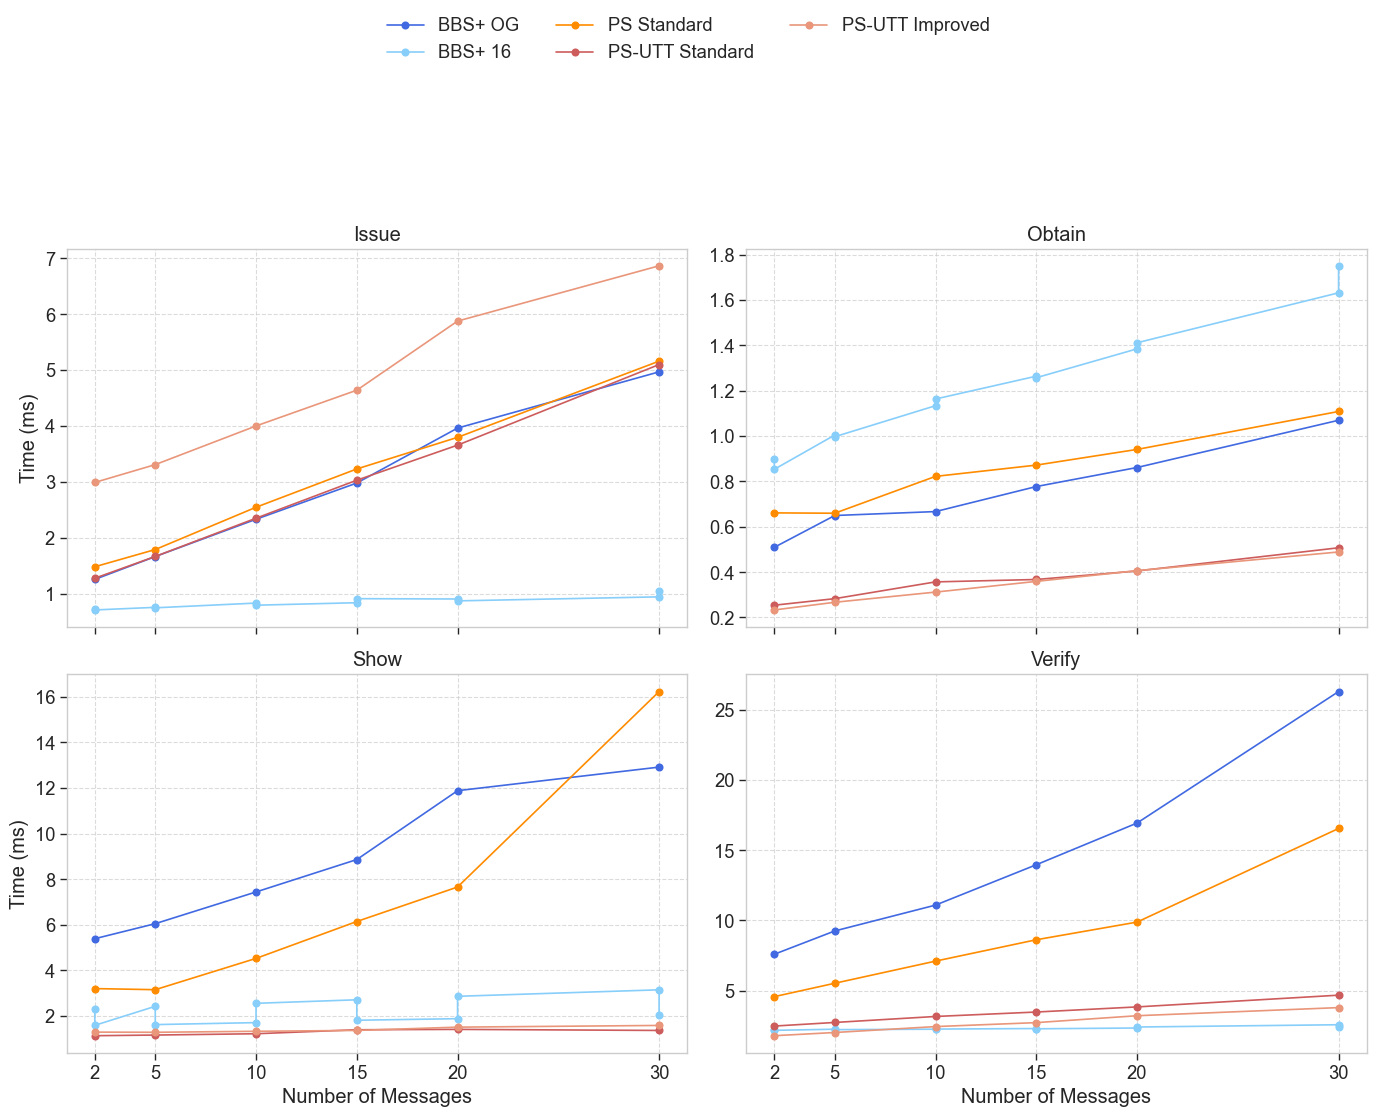
\includegraphics[width=1\linewidth]{comparison-line-graph.png}
    \caption{Performance Comparison of Anonymous Credential Schemes}
    
\end{figure}

\begin{figure}
    \centering
    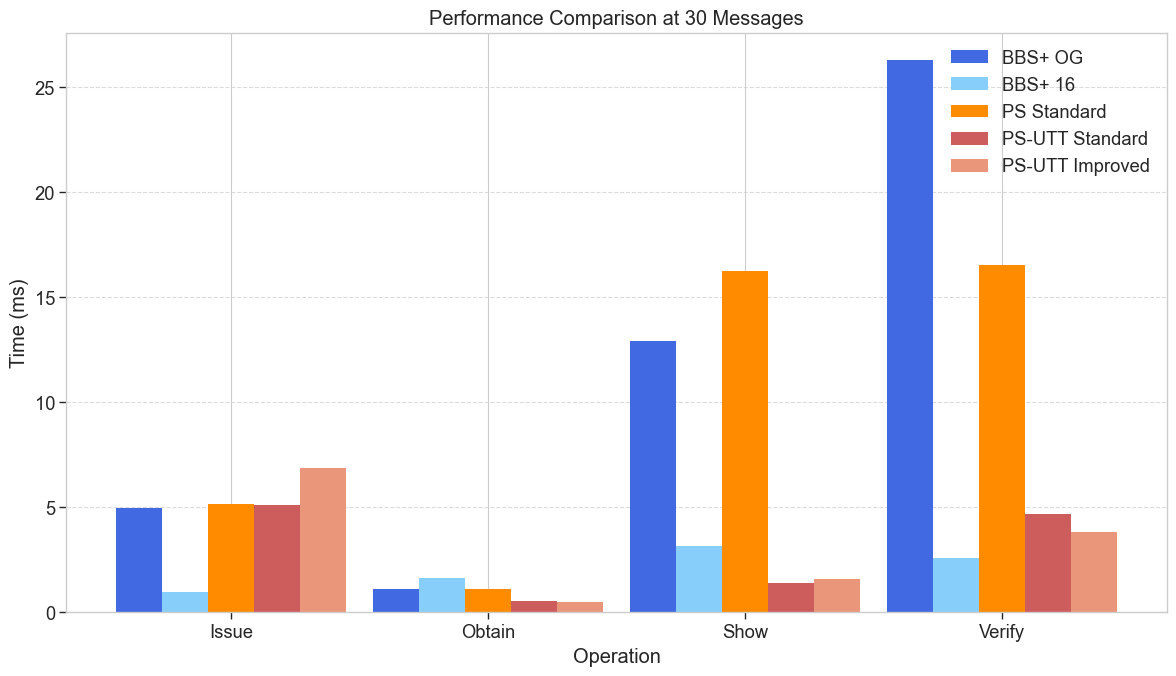
\includegraphics[width=0.7\linewidth]{performance-30.png}
    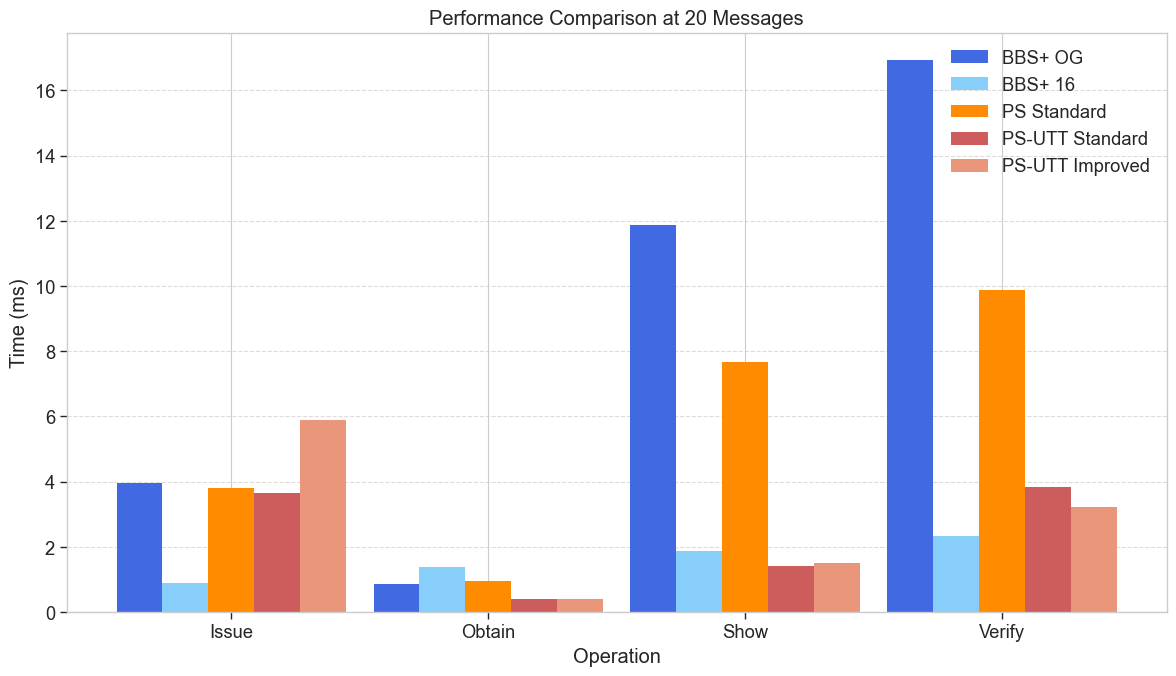
\includegraphics[width=0.7\linewidth]{performance-20.png}
    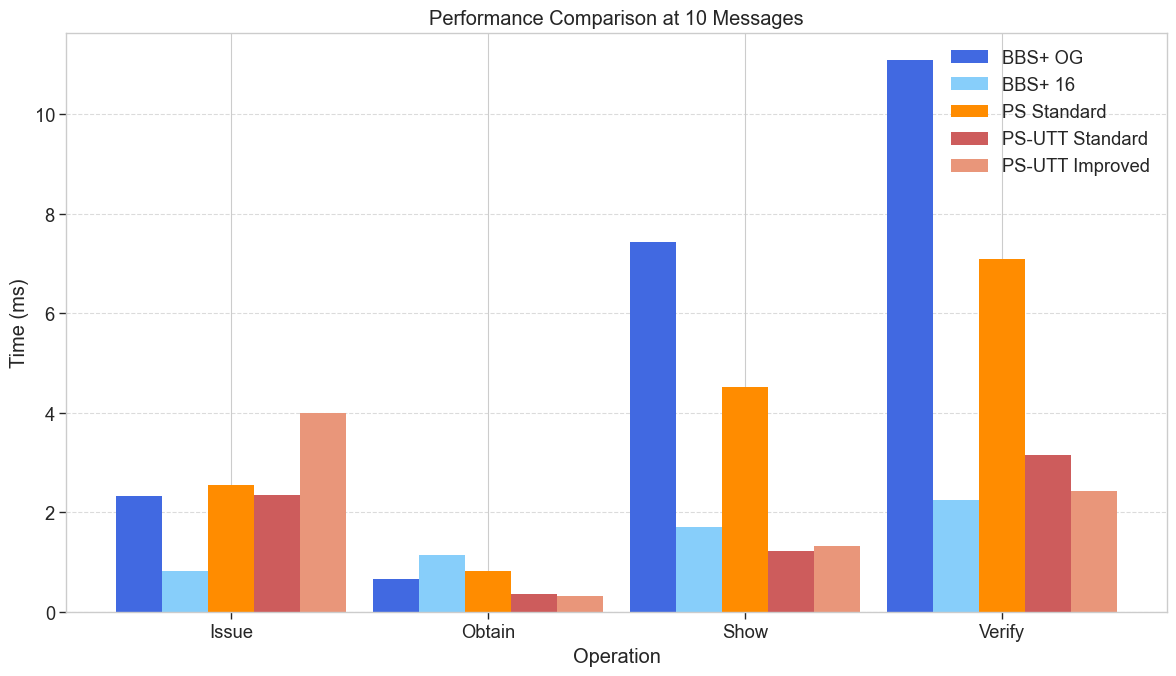
\includegraphics[width=0.7\linewidth]{performance-10.png}
     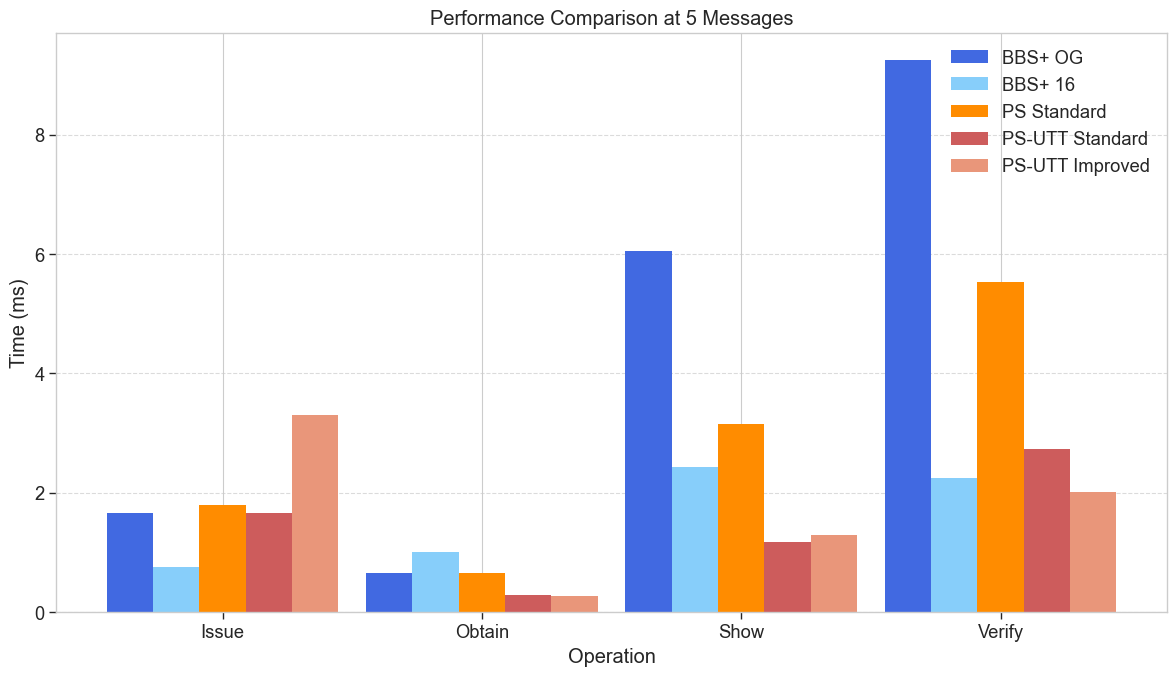
\includegraphics[width=0.7\linewidth]{performance-5.png}
    \caption{Performance Comparison of Anonymous Credential Schemes}
    
\end{figure}




% \subsubsection{Case Study: Credential Expiration Verification}

% To demonstrate the practical impact of our optimizations, we compared our approach against alternative systems for the common use case of verifying credential expiration. Table~\ref{tab:expiry-comparison} presents the results for generating and verifying a proof that a credential has not expired.

% \begin{table}[htbp]
% \centering
% \caption{Performance Comparison for Credential Expiration Verification}
% \label{tab:expiry-comparison}
% \begin{tabular}{lrrr}
% \toprule
% \textbf{Approach} & \textbf{Show (ms)} & \textbf{Verify (ms)} & \textbf{Proof Size} \\
% \midrule
% Simple Possession & 2 & 2 & 424B \\
% Expiry (ZK-Creds) & 50 & \multirow{3}{*}{$\left\}5\text{ ms}\right.$} & \multirow{3}{*}{744B} \\
% Linkable Show (ZK-Creds) & 41 &  &  \\
% Rate Limiting (ZK-Creds) & 58 &  &  \\
% \textbf{Our Approach} & \textbf{1.3} & \textbf{2.0} & \textbf{512B} \\
% \bottomrule
% \end{tabular}
% \end{table}

% Our evaluation reveals that our system can verify a credential's expiry status in just 3.3ms (combined Show+Verify), compared to 45-55ms for ZK-Creds approaches—a performance improvement of over 13×. This dramatic difference highlights how our optimized signature scheme and sigma protocol enables efficient predicate verification without sacrificing privacy.

% Importantly, while general-purpose zero-knowledge systems provide flexibility, they introduce substantial computational overhead that makes interactive verification scenarios impractical. Our approach achieves similar expressiveness with dramatically better performance for the most common credential verification operations.
















